\documentclass[12pt]{article}
\usepackage{graphicx}
\usepackage{setspace}
\usepackage{fancyhdr}
\usepackage{amssymb}
\usepackage{xcolor}
\usepackage{amsmath}
\usepackage{svg}
\usepackage{graphicx}
\usepackage[a4paper, margin=1in]{geometry}
\pagestyle{fancy}
\lhead{Wavelet Implementation for 1D and 2D Data}
\rhead{Aliakbar Zarkoob}

\begin{document}
	
	\begin{titlepage}
		\begin{center}
			
			
\includegraphics[height=4cm]{University_of_Tehran_Transparent_BW_logo.png} \hfill
			
\includegraphics[height=4cm]{Fanni_Alt_BW_Logo.png}
			
			\vspace{1cm}
			
			\Large \textbf{School of Surveying and Geospatial Engineering}\\
			\large {Department of Geodesy and Hydrography}
			
			\vspace{3cm}
			
			\huge \textbf{Wavelet Implementation for 1D and 2D Data}
			
			\vspace{1.5cm}
			
			\Large \textbf{Author:}\\
			\Large Aliakbar Zarkoob
			
			\vspace{2cm}
			
			\Large \textbf{Professor:}\\
			Dr. Abdolreza Safari
			
			\vfill
			
			\large {Autumn 2024}
			
		\end{center}
	\end{titlepage}
	
	
	\section{Introduction}
	
	Wavelet analysis has become a fundamental tool in signal processing, data compression, and various fields of scientific research due to its ability to reveal information across different scales and resolutions. Unlike Fourier analysis, which primarily focuses on the frequency domain, wavelet transforms allow for simultaneous analysis in both the time/space and frequency domains. This dual-domain capability makes wavelets especially useful for analyzing non-stationary signals or images where features of interest may vary in size or frequency.
	
	Wavelet transforms can be applied to both one-dimensional (1D) and two-dimensional (2D) data, providing significant versatility. In 1D data, wavelet analysis is commonly used for tasks such as noise reduction and feature extraction in time-series data, while in 2D data, it is widely utilized for image compression, edge detection, and texture analysis. 

	\section{One-Dimensional Wavelets}
	
	Assuming that a 1D signal like equation \ref{eq:signal} exists, where $n$ is a power of 2. The aim in wavelet transform is to reconstruct the signal with smooth and detail parts, as shown in equation \ref{eq:1d_wavelet_transform}. these two parts can be calculated by the equations \ref{eq:1d_parts} and \ref{eq:1d_parts_n}, where $k$ indicates the level of decomposition.
	
	\begin{equation}
		f=(f_1,f_2,f_3,...,f_n)
		\label{eq:signal}
	\end{equation}
	
	\begin{equation}
		f=\sum_{i=1} \langle f, V_{i}^1 \rangle V_{i}^1 + \sum_{j=1}^{\frac{N}{2^j}}\sum_{i=1}\langle f, W_{i}^j \rangle W_{i}^j
		\label{eq:1d_wavelet_transform}
	\end{equation}
	
	\begin{equation}
		\begin{aligned}
		s_i^k &= f \cdot V_i^k \\
		d_i^k &= f \cdot W_i^k
		\end{aligned}
		\label{eq:1d_parts}
	\end{equation}
	
		\begin{equation}
		\begin{aligned}
			S^k &= s_1^k \cdot V_1^k + s_2^k \cdot V_2^k + \dots + s_i^k \cdot V_i^k \\
			D^k &= d_1^k \cdot W_1^k + d_2^k \cdot W_2^k + \dots + d_i^k \cdot W_i^k
		\end{aligned}
		\label{eq:1d_parts_n}
	\end{equation}
	
	$V$ and $W$ in the equation \ref{eq:1d_wavelet_transform} are basis vectors that create the smooth and detail spaces. These basis vectors are created based on scaling function $\phi(x)$ and wavelet function $\psi(x)$. How these two functions are defined, separates different types of wavelets. In this report, 5 types of wavelets are used (Haar, Daubechies4, Daubechies6, Mexican Hat and Symlet2).

	\subsection{Haar Wavelet}
	
	The scaling and wavelet function for Haar wavelet is defined as below. The basis vectors $V$ and $W$ are created with coefficients $h$ and $g$. These basis vectors for the first level of decomposition are shown in the equations \ref{eq:v_haar} and \ref{eq:w_haar}.
	
	\begin{equation}
		\phi(x) = 
		\begin{cases} 
			1 &  0 \leq x < 1 \\
			0 & \text{otherwise}
		\end{cases}
		\label{eq:scalingfunc_haar}
	\end{equation}
	
	\begin{equation}
		\psi(x) = 
		\begin{cases} 
			1 &  0 \leq x < \frac{1}{2} \\
			-1 &  \frac{1}{2} \leq x < 1 \\
			0 & \text{otherwise}
		\end{cases}
		\label{eq:waveletfunc_haar}
	\end{equation}
	
	\begin{equation}
		\begin{aligned}
			V_1^1 &= (h_0, h_1, 0, 0, \dots, 0, 0) \\
			V_2^1 &= (0, 0, h_0, h_1, \dots, 0, 0) \\
			&\vdots \\
			V_{\frac{n}{2}}^1 &= (0, 0, 0, 0, \dots, h_0, h_1)\\
			\\
			h_0 &= \frac{1}{\sqrt{2}} \;\;,\;\; h_1 = \frac{1}{\sqrt{2}}
		\end{aligned}
		\label{eq:v_haar}
	\end{equation}
	
	\begin{equation}
		\begin{aligned}
			W_1^1 &= (g_0, g_1, 0, 0, \dots, 0, 0) \\
			W_2^1 &= (0, 0, g_0, g_1, \dots, 0, 0) \\
			&\vdots \\
			W_{\frac{n}{2}}^1 &= (0, 0, 0, 0, \dots, g_0, g_1)\\
			\\
			g_0 &= \frac{1}{\sqrt{2}} \;\;,\;\; g_1 = -\frac{1}{\sqrt{2}}
		\end{aligned}
		\label{eq:w_haar}
	\end{equation}
	
	\subsection{Daubechies4 Wavelet}
	
	The basis vectors $V$ and $W$ for the first level of decomposition are created as shown in the equations \ref{eq:v_db4} and \ref{eq:w_db4}.
	
	\begin{equation}
		\begin{aligned}
			V_1^1 &= (h_0, h_1, h_2, h_3, 0, 0, 0, 0 \dots, 0, 0, 0, 0) \\
			V_2^1 &= (0, 0, h_0, h_1, h_2, h_3, 0, 0, \dots, 0, 0, 0, 0) \\
			&\vdots \\
			V_{\frac{n}{2}}^1 &= (h_2, h_3 ,0 ,0 ,0 ,0, 0, 0, \dots, 0, 0, h_0, h_1)\\
			\\
			h_0 = \frac{1+\sqrt3}{4\sqrt{2}}& \;,\; h_1 = \frac{3+\sqrt3}{4\sqrt{2}} \;,\; h_2 = \frac{3-\sqrt3}{4\sqrt{2}} \;,\; h_3 = \frac{1-\sqrt3}{4\sqrt{2}}
		\end{aligned}
		\label{eq:v_db4}
	\end{equation}
	
	\begin{equation}
		\begin{aligned}
			W_1^1 &= (g_0, g_1, g_2, g_3, 0, 0, 0, 0 \dots, 0, 0, 0, 0) \\
			W_2^1 &= (0, 0, g_0, g_1, g_2, g_3, 0, 0, \dots, 0, 0, 0, 0) \\
			&\vdots \\
			W_{\frac{n}{2}}^1 &= (g_2, g_3 ,0 ,0 ,0 ,0, 0, 0, \dots, 0, 0, g_0, g_1)\\
			\\
			g_0 &= h_3 \;,\; g_1 = -h_2 \;,\; g_2 = h_1 \;,\; g_3 = -h_0
		\end{aligned}
		\label{eq:w_db4}
	\end{equation}
	
	\subsection{Daubechies6 Wavelet}
	
	The basis vectors $V$ and $W$ for other wavelets are created in the same manner, but the  $h$ and $g$ coefficients are different. these coefficients for Daubechies6 are shown in the equations \ref{eq:h_db6} and \ref{eq:g_db6}.
	
	\begin{equation}
		\begin{aligned}
		h_0 &= 0.3326705529500826 \;,\; h_1 = 0.8068915093110928 \\
		h_2 &= 0.4598775021184915 \;,\; h_3 = -0.1350110200102546 \\
		h_4 &= -0.0854412738822415 \;,\; h_5 = 0.0352262918857095
		\end{aligned}
		\label{eq:h_db6}
	\end{equation}
	
	\begin{equation}
		\begin{aligned}
		g_0 &= h_5 \;,\; g_1 = -h_4 \;,\; g_2 = h_3 \\
		g_3 &= -h_2 \;,\; g_4 = h_1 \;,\; g_5 = -h_0
		\end{aligned}
		\label{eq:g_db6}
	\end{equation}
	
	\subsection{Mexican Hat Wavelet}
	The  $h$ and $g$ coefficients for Mexican Hat Wavelet are shown in the equations \ref{eq:h_mh} and \ref{eq:g_mh}.
	
	\begin{equation}
		\begin{aligned}
			h_0 = \frac{1-\sqrt7}{16\sqrt2} \;,\; h_1 &= \frac{5+\sqrt7}{16\sqrt2} \;,\; h_2 = \frac{14+2\sqrt7}{16\sqrt2} \\
			h_3 = \frac{14-2\sqrt7}{16\sqrt2} \;,\; h_4 &= \frac{1-\sqrt7}{16\sqrt2} \;,\; h_5 = \frac{-3+2\sqrt7}{16\sqrt2} \;,\;
		\end{aligned}
		\label{eq:h_mh}
	\end{equation}
	
	\begin{equation}
		\begin{aligned}
			g_0 &= h_5 \;,\; g_1 = -h_4 \;,\; g_2 = h_3 \\
			g_3 &= -h_2 \;,\; g_4 = h_1 \;,\; g_5 = -h_0
		\end{aligned}
		\label{eq:g_mh}
	\end{equation}
	
	\subsection{Symlet2 Wavelet}
	
	The  $h$ and $g$ coefficients for Mexican Hat Wavelet are shown in the equations \ref{eq:h_sym2} and \ref{eq:g_sym2}.
	
	\begin{equation}
		\begin{aligned}
			h_0 &= 0.3326705529500826 \;,\; h_1 = 0.8068915093133388 \\
			h_2 &= 0.4598775021184915 \;,\; h_3 = -0.1350110200102546 \\
			h_4 &= -0.0854412738820267 \;,\; h_5 = 0.0352262918857095
		\end{aligned}
		\label{eq:h_sym2}
	\end{equation}
	
	\begin{equation}
		\begin{aligned}
			g_0 &= -h_5 \;,\; g_1 = h_4 \;,\; g_2 = -h_3 \\
			g_3 &= h_2 \;,\; g_4 = -h_1 \;,\; g_5 = h_0
		\end{aligned}
		\label{eq:g_sym2}
	\end{equation}
	
	\section{Two-Dimensional Wavelets}
	
	Assuming that an $m\times n$ image like equation \ref{eq:f_image} exists, where $m$ and $n$ are powers of 2. Unlike the case of 1D signal that two parts of smooth and detail existed, here there are four parts, shown in equation \ref{eq:2d_parts} where $k$ indicates the decomposition level.
	
	\begin{equation}
		f = 
		\begin{bmatrix}
			f_{11} & f_{12} & \dots & f_{1n} \\
			f_{21} & f_{22} & \dots & f_{2n} \\
			\vdots & \vdots & \ddots & \vdots \\
			f_{m1} & f_{m2} & \dots & f_{mn} 
		\end{bmatrix}
		\label{eq:f_image}
	\end{equation}
		
	\begin{equation}
		\begin{bmatrix}
		\begin{array}{c|c}
			ss^k & sd^k \\
			\hline
			ds^k & dd^k
		\end{array}
		\end{bmatrix}
	\end{equation}
	
	The basis elements for creating these four parts are the outer product of the $V$ and $W$ vectors defined in one-dimensional wavelets. These four parts can be constructed with the equations \ref{eq:2d_parts} and \ref{eq:2d_parts_n}.
	
	\begin{equation}
		\begin{aligned}
		ss_{ij}^k &= \; f \cdot (V_{ij}^k \otimes V_{ij}^k) \\
		sd_{ij}^k &= \; f \cdot (V_{ij}^k \otimes W_{ij}^k) \\
		ds_{ij}^k &= \; f \cdot (W_{ij}^k \otimes V_{ij}^k) \\
		dd_{ij}^k &= \; f \cdot (W_{ij}^k \otimes W_{ij}^k)
		\end{aligned}
		\label{eq:2d_parts}
	\end{equation}

	\begin{equation}
		\begin{aligned}
		SS^k &= ss_{11}^k V_1^k \otimes V_1^k + ss_{12}^k V_1^k \otimes V_2^k + \dots + ss_{\frac{m}{2}\frac{n}{2}}^k V_{\frac{m}{2}}^k \otimes V_{\frac{n}{2}}^k \\
		SD^k &= sd_{11}^k V_1^k \otimes W_1^k + sd_{12}^k V_1^k \otimes W_2^k + \dots + sd_{\frac{m}{2}\frac{n}{2}}^k V_{\frac{m}{2}}^k \otimes W_{\frac{n}{2}}^k \\
		DS^k &= ds_{11}^k W_1^k \otimes V_1^k + ds_{12}^k W_1^k \otimes V_2^k + \dots + ds_{\frac{m}{2}\frac{n}{2}}^k W_{\frac{m}{2}}^k \otimes V_{\frac{n}{2}}^k \\
		DD^k &= dd_{11}^k W_1^k \otimes W_1^k + dd_{12}^k W_1^k \otimes W_2^k + \dots + dd_{\frac{m}{2}\frac{n}{2}}^k W_{\frac{m}{2}}^k \otimes W_{\frac{n}{2}}^k
		\end{aligned}
		\label{eq:2d_parts_n}
	\end{equation}
	
	\section{Implementations}
	
	\subsection{One-Dimensional}
	
	\subsubsection{Noise Reduction}
	
	A 1D signal is created with the equation \ref{eq:1d_signal}. Then white noise with the standard deviation of 1 is added to the signal. The created signal before and after adding noise is shown in the figure \ref{fig:1d_signal}.
	
	\begin{equation}
%		f(x)=2x^2 + 10\sin(4x) + \cos^2(x^2)
		f(x) = 25sin(2\pi(0.5 +5x)x)
		\label{eq:1d_signal}
	\end{equation}
	
	\begin{figure}[!h]
		\centering
		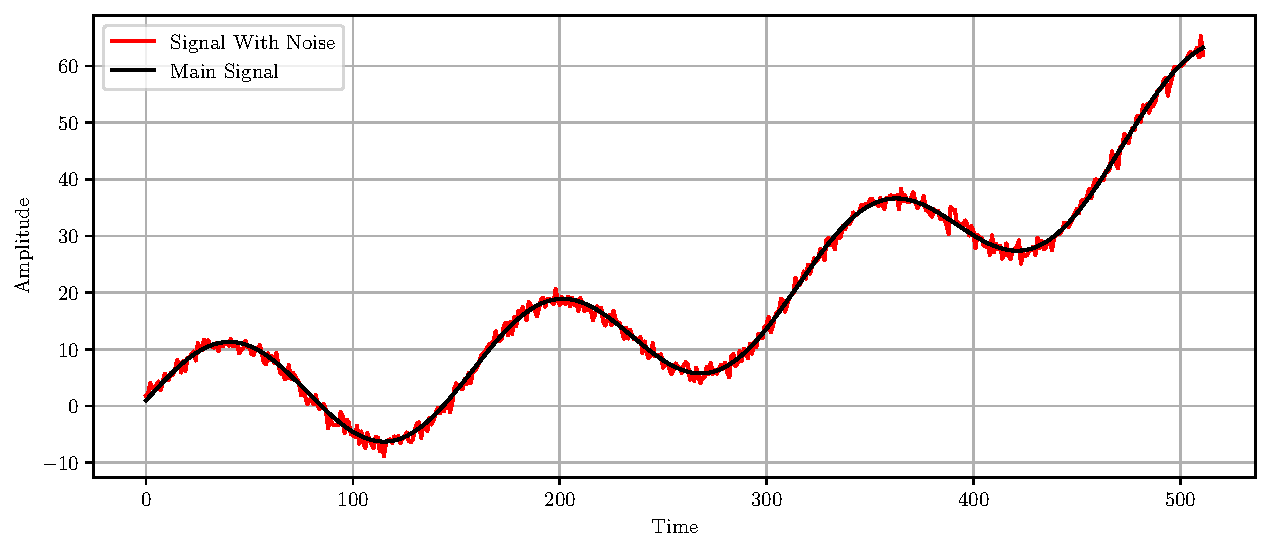
\includegraphics[height=7cm]{../Tests/Outputs/1D_Signal.pdf}
		\caption{Constructed 1D signal, before and after adding white noise.}
		\label{fig:1d_signal}
	\end{figure}
	
	The results for 5 mentioned wavelets are shown in the figures \ref{fig:1d_haar} to \ref{fig:1d_sym2}.
	
	\begin{figure}[!h]
		\centering
		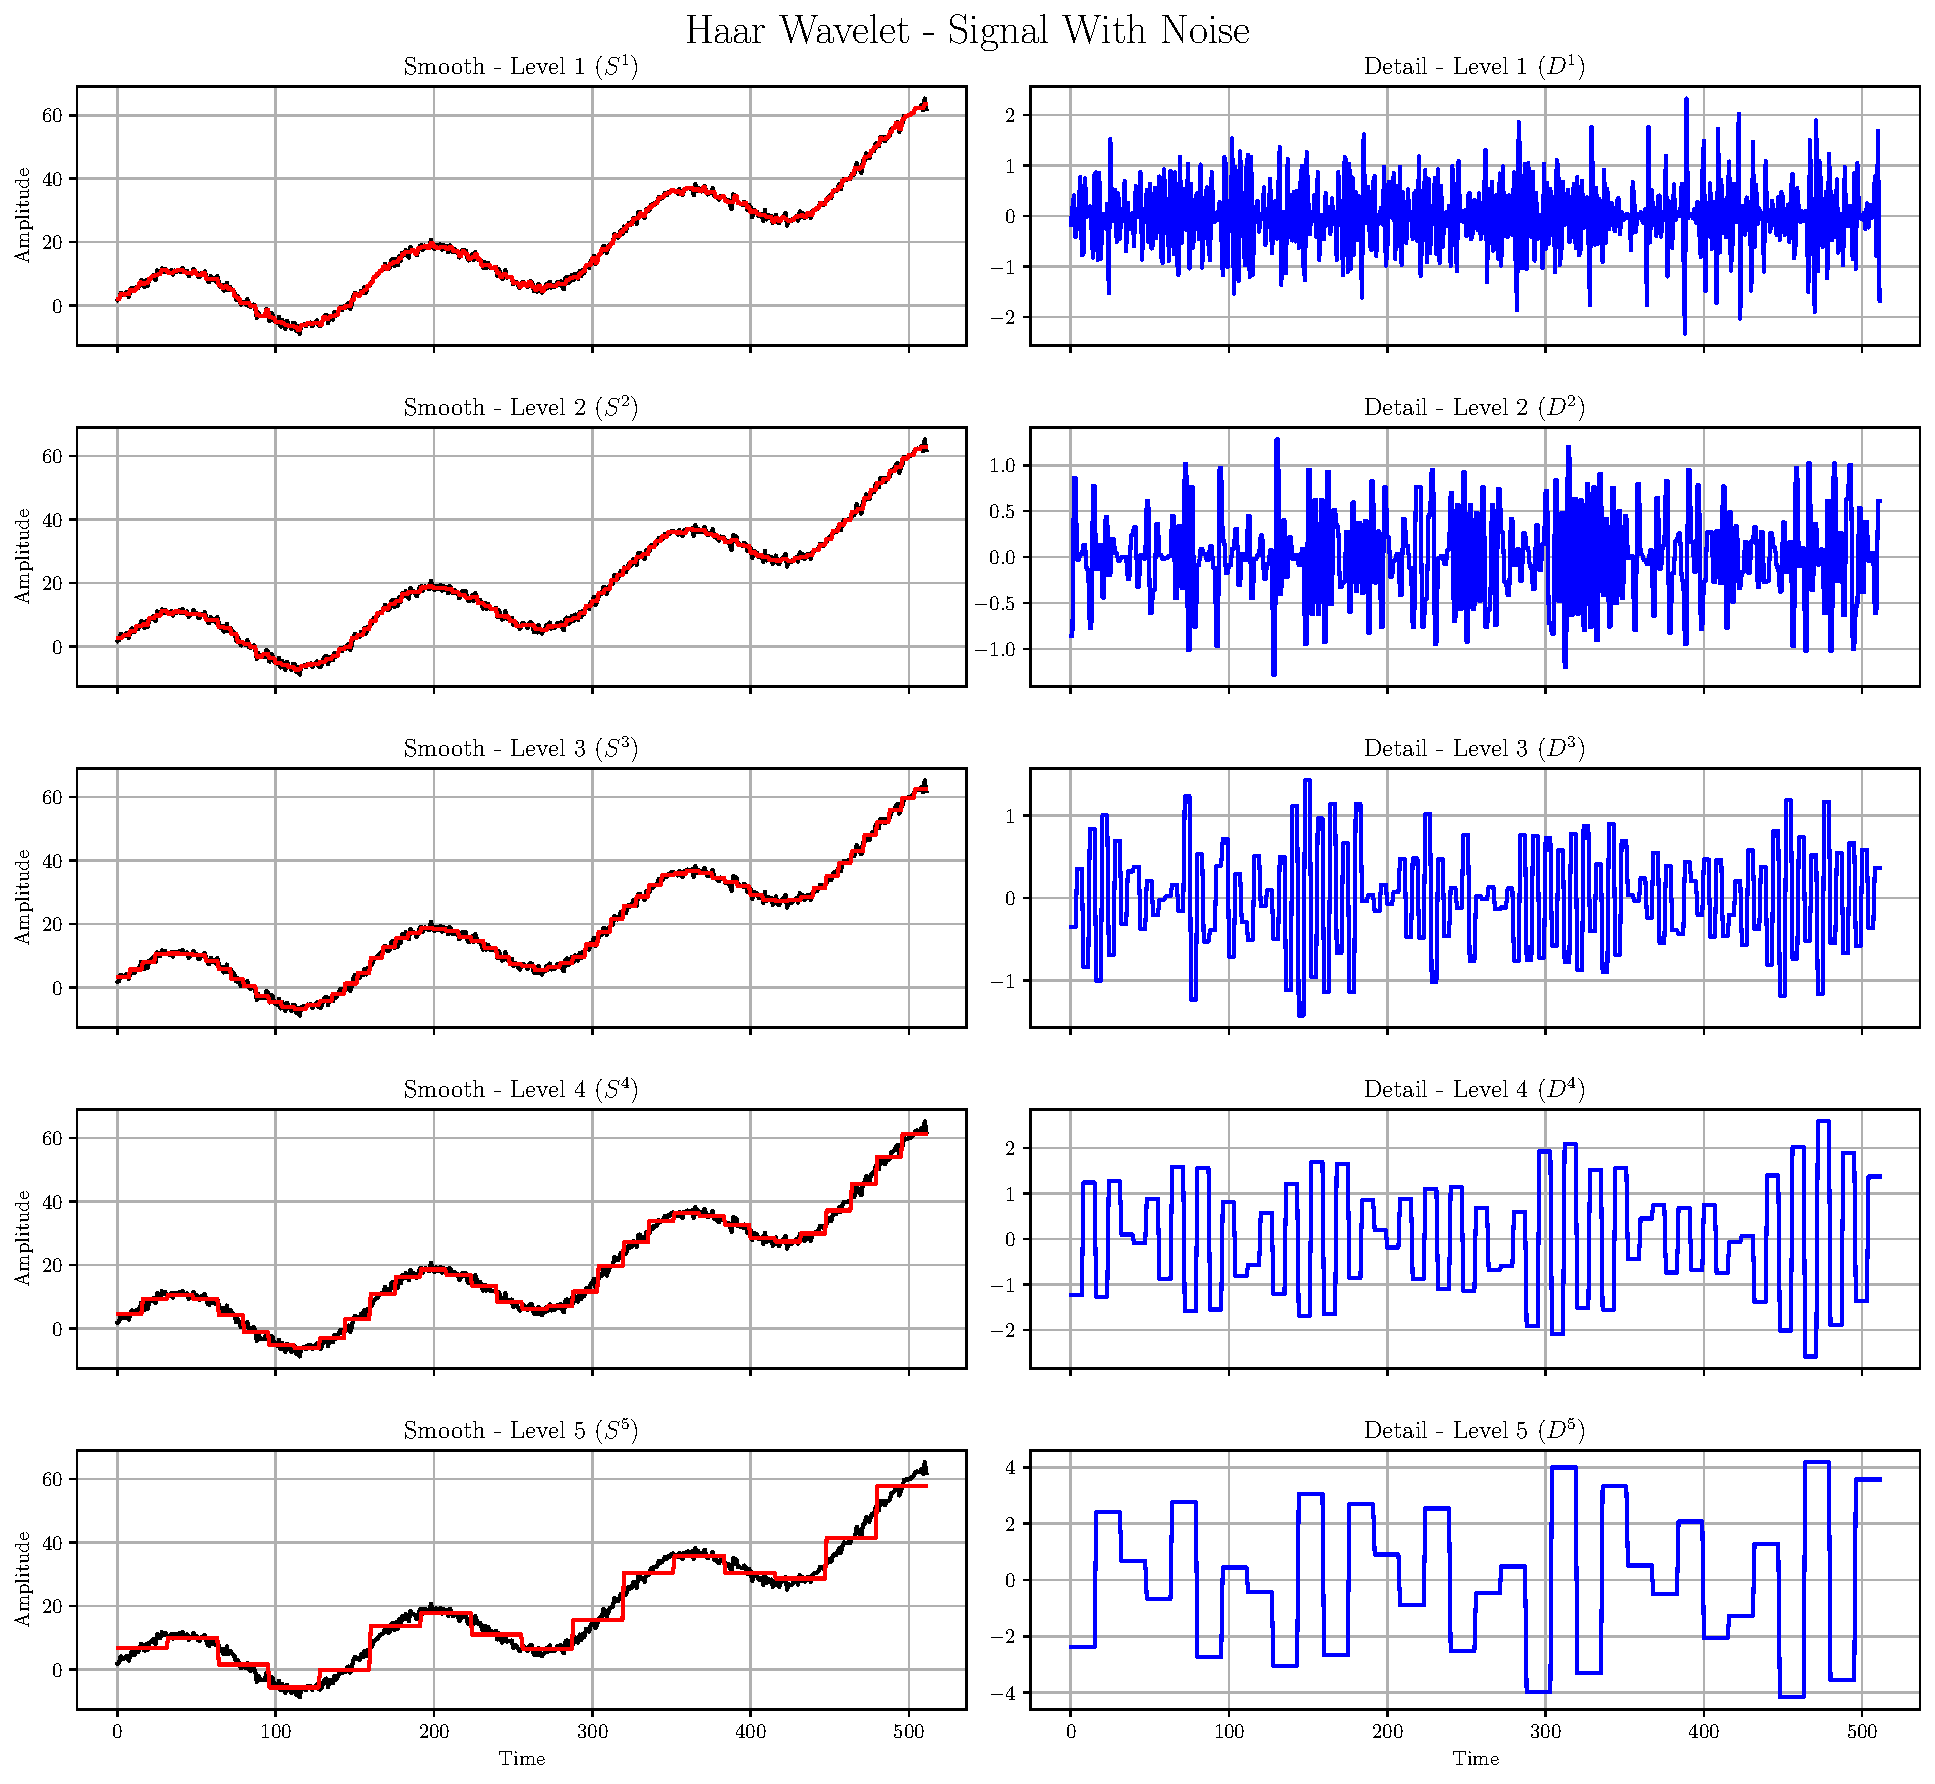
\includegraphics[height=11cm]{../Tests/Outputs/HaarWavelet_SignalWithNoise.pdf}
		\caption{Results of Haar wavelet on the simulated signal.}
		\label{fig:1d_haar}
	\end{figure}

	\begin{figure}[!h]
		\centering
		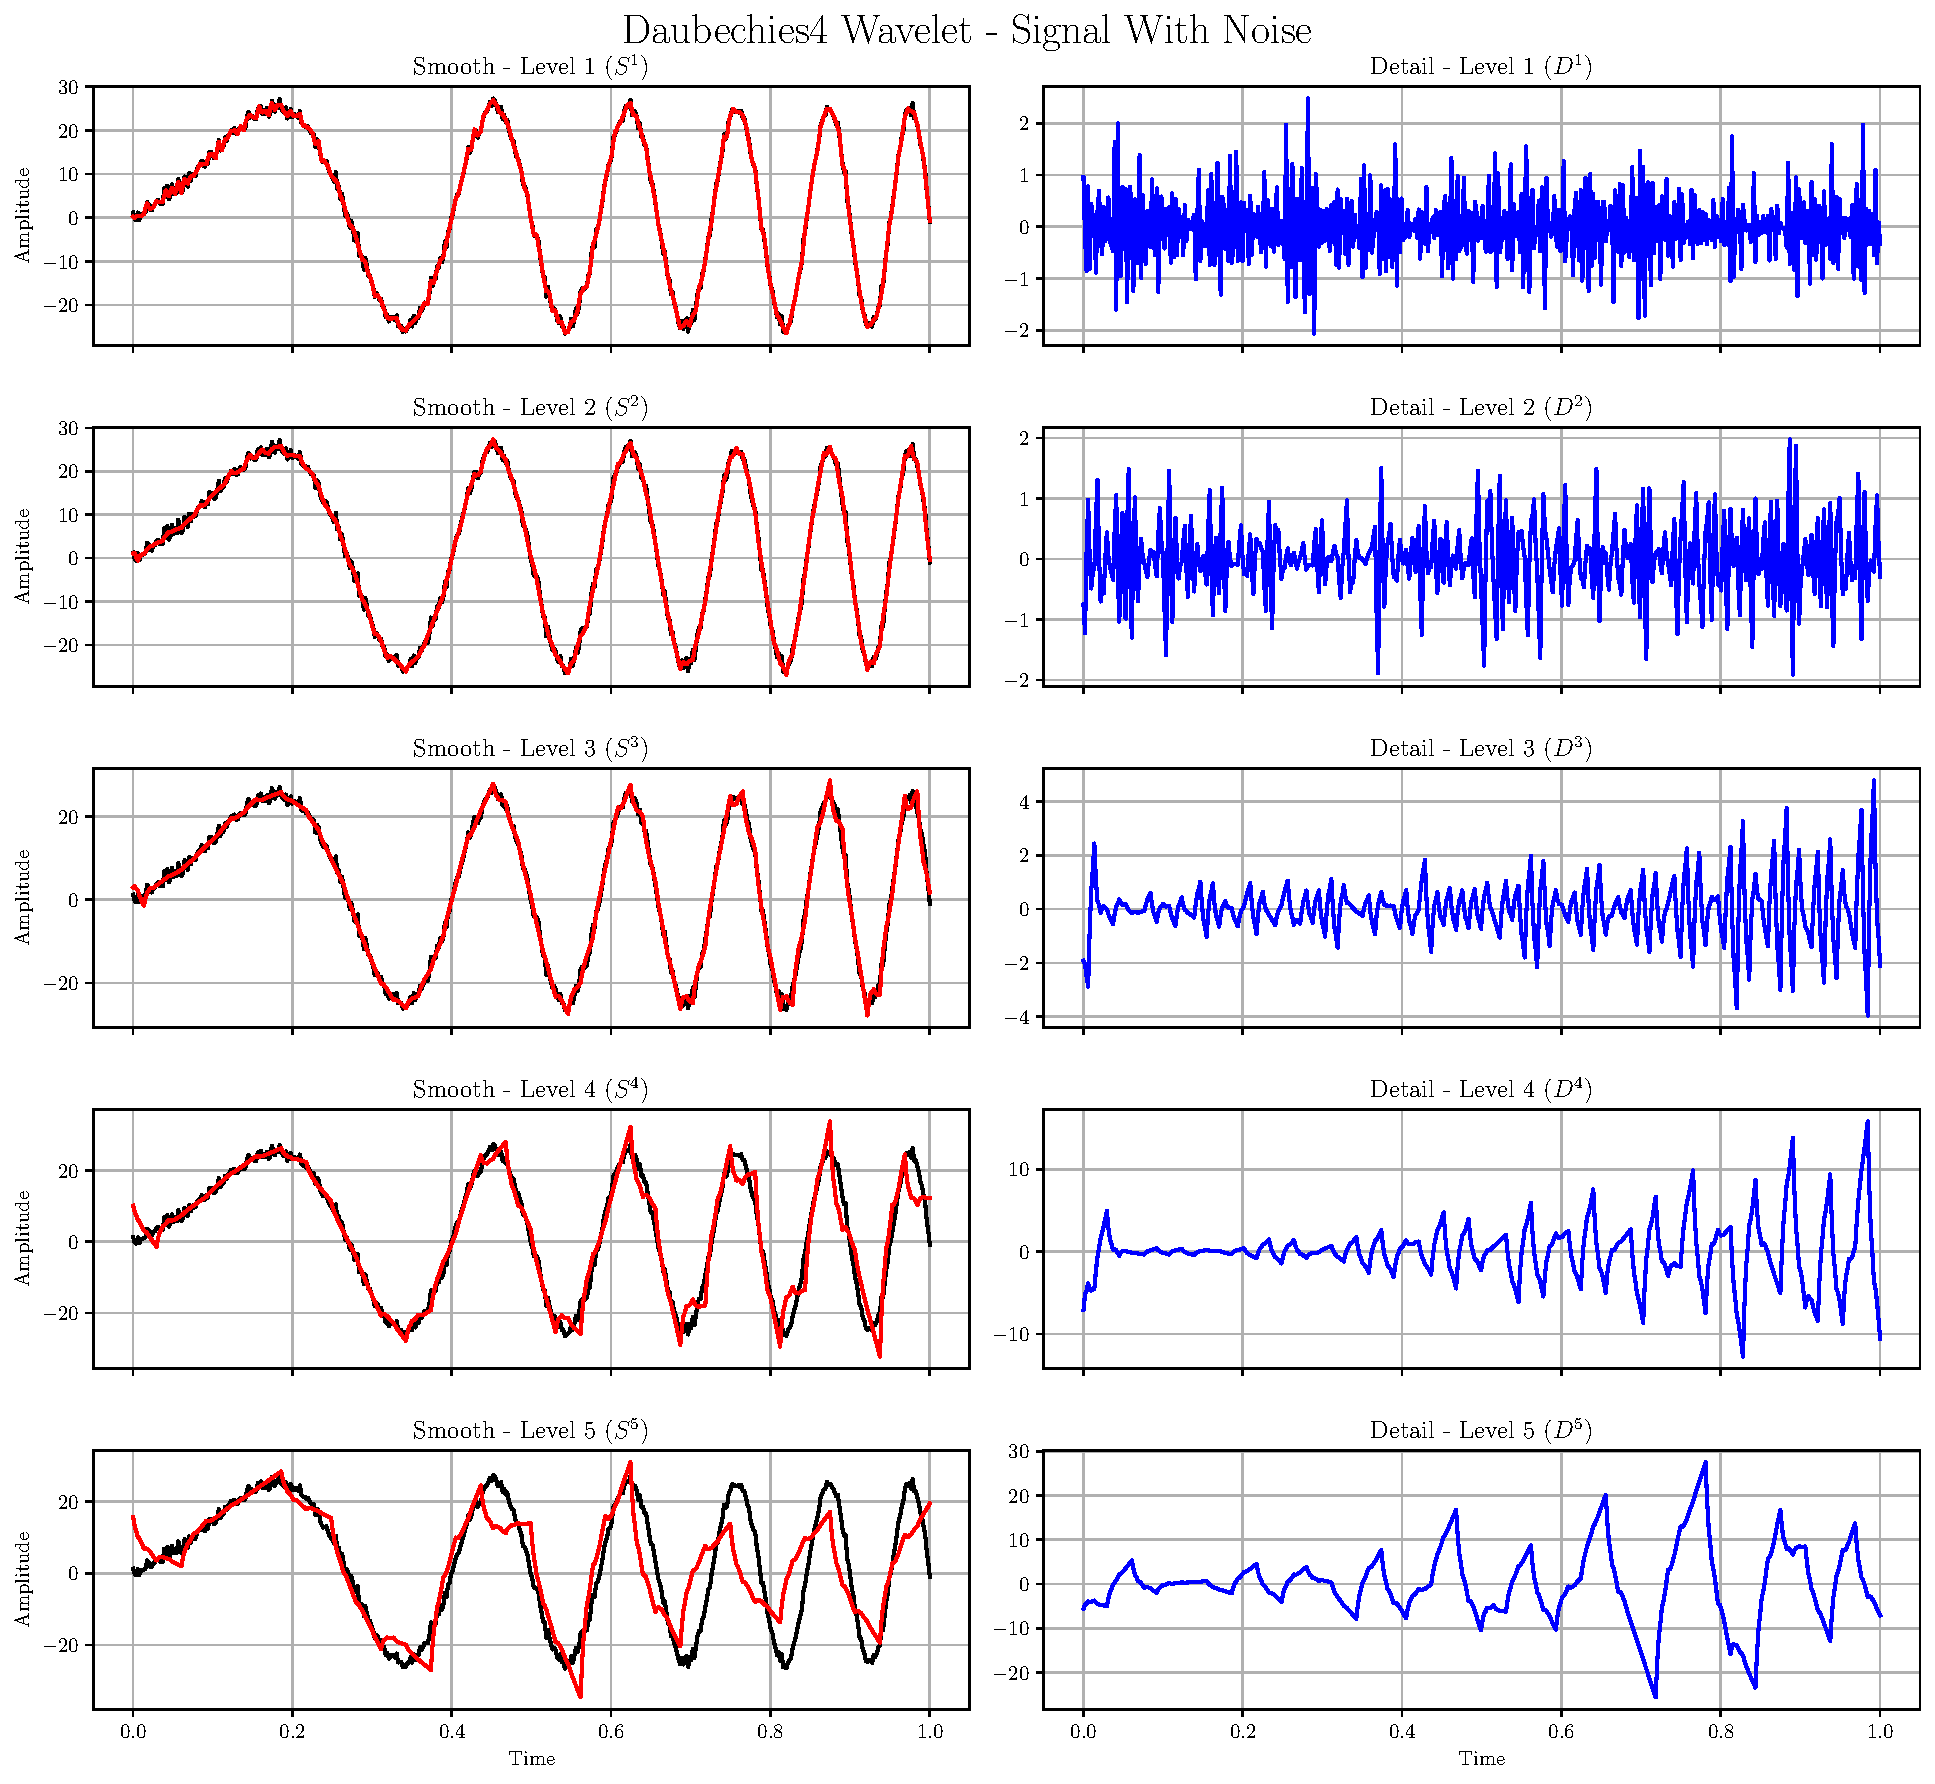
\includegraphics[height=11cm]{../Tests/Outputs/Daubechies4Wavelet_SignalWithNoise.pdf}
		\caption{Results of Daubechies4 wavelet on the simulated signal.}
		\label{fig:1d_db4}
	\end{figure}	
	
	\begin{figure}[!h]
		\centering
		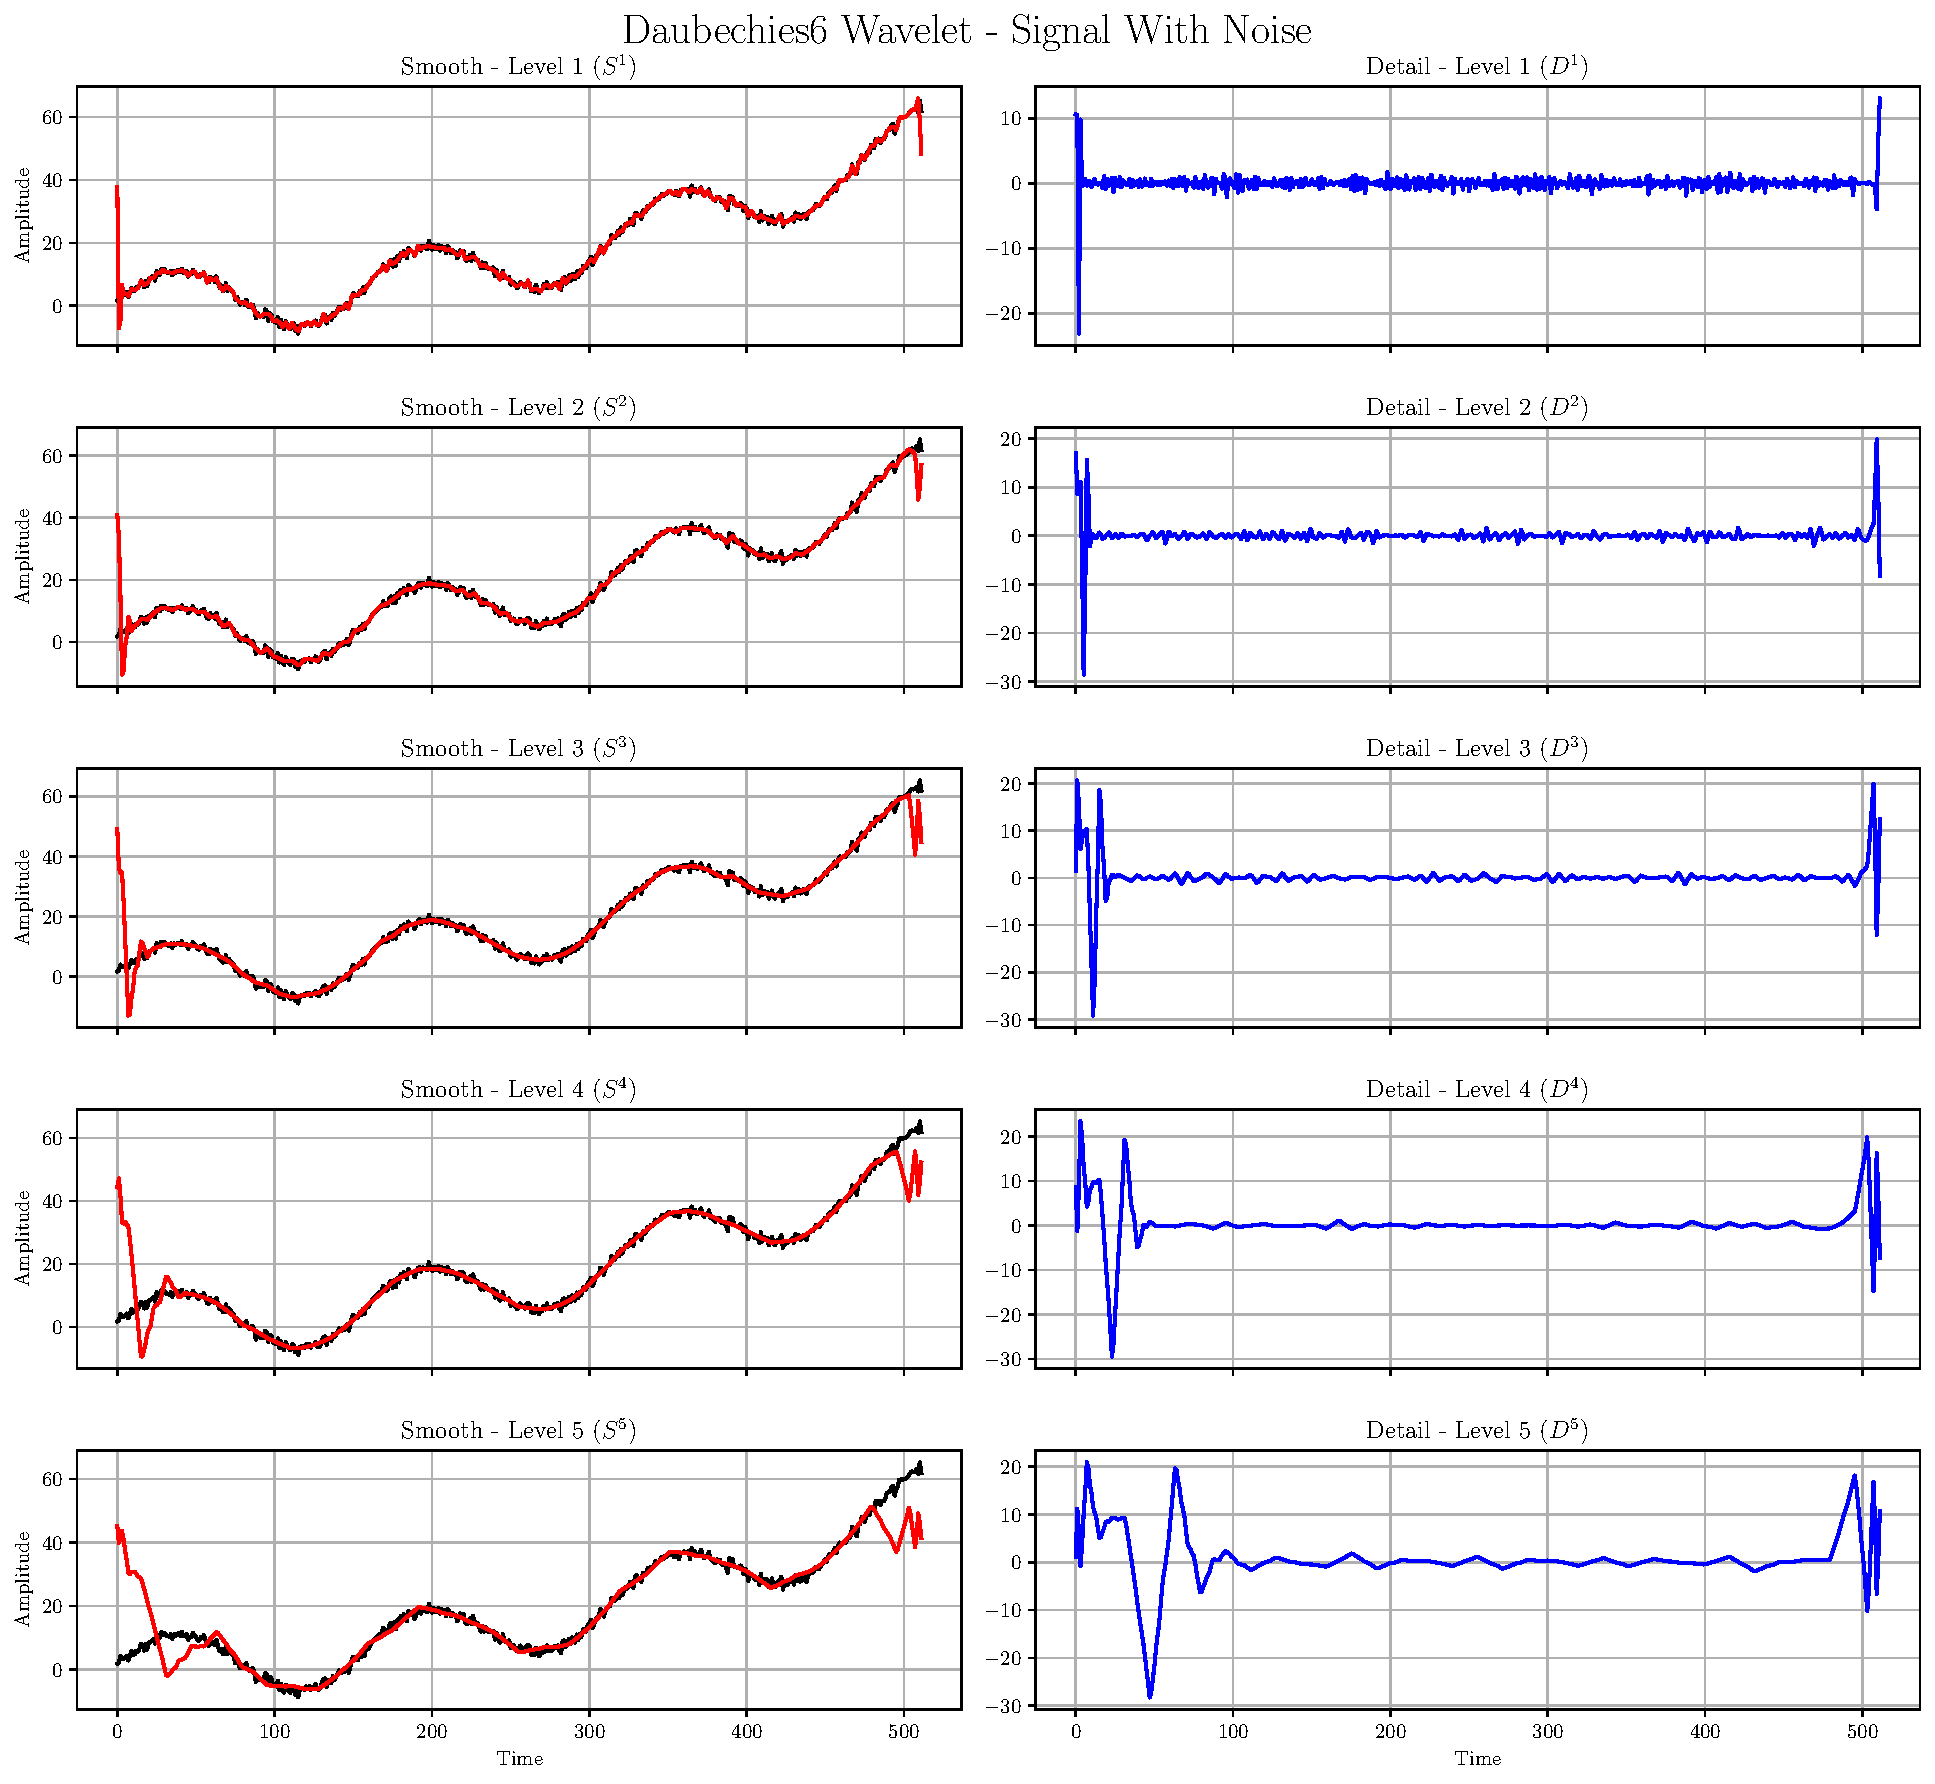
\includegraphics[height=11cm]{../Tests/Outputs/Daubechies6Wavelet_SignalWithNoise.pdf}
		\caption{Results of Daubechies6 wavelet on the simulated signal.}
		\label{fig:1d_db6}
	\end{figure}
	
	\begin{figure}[!h]
		\centering
		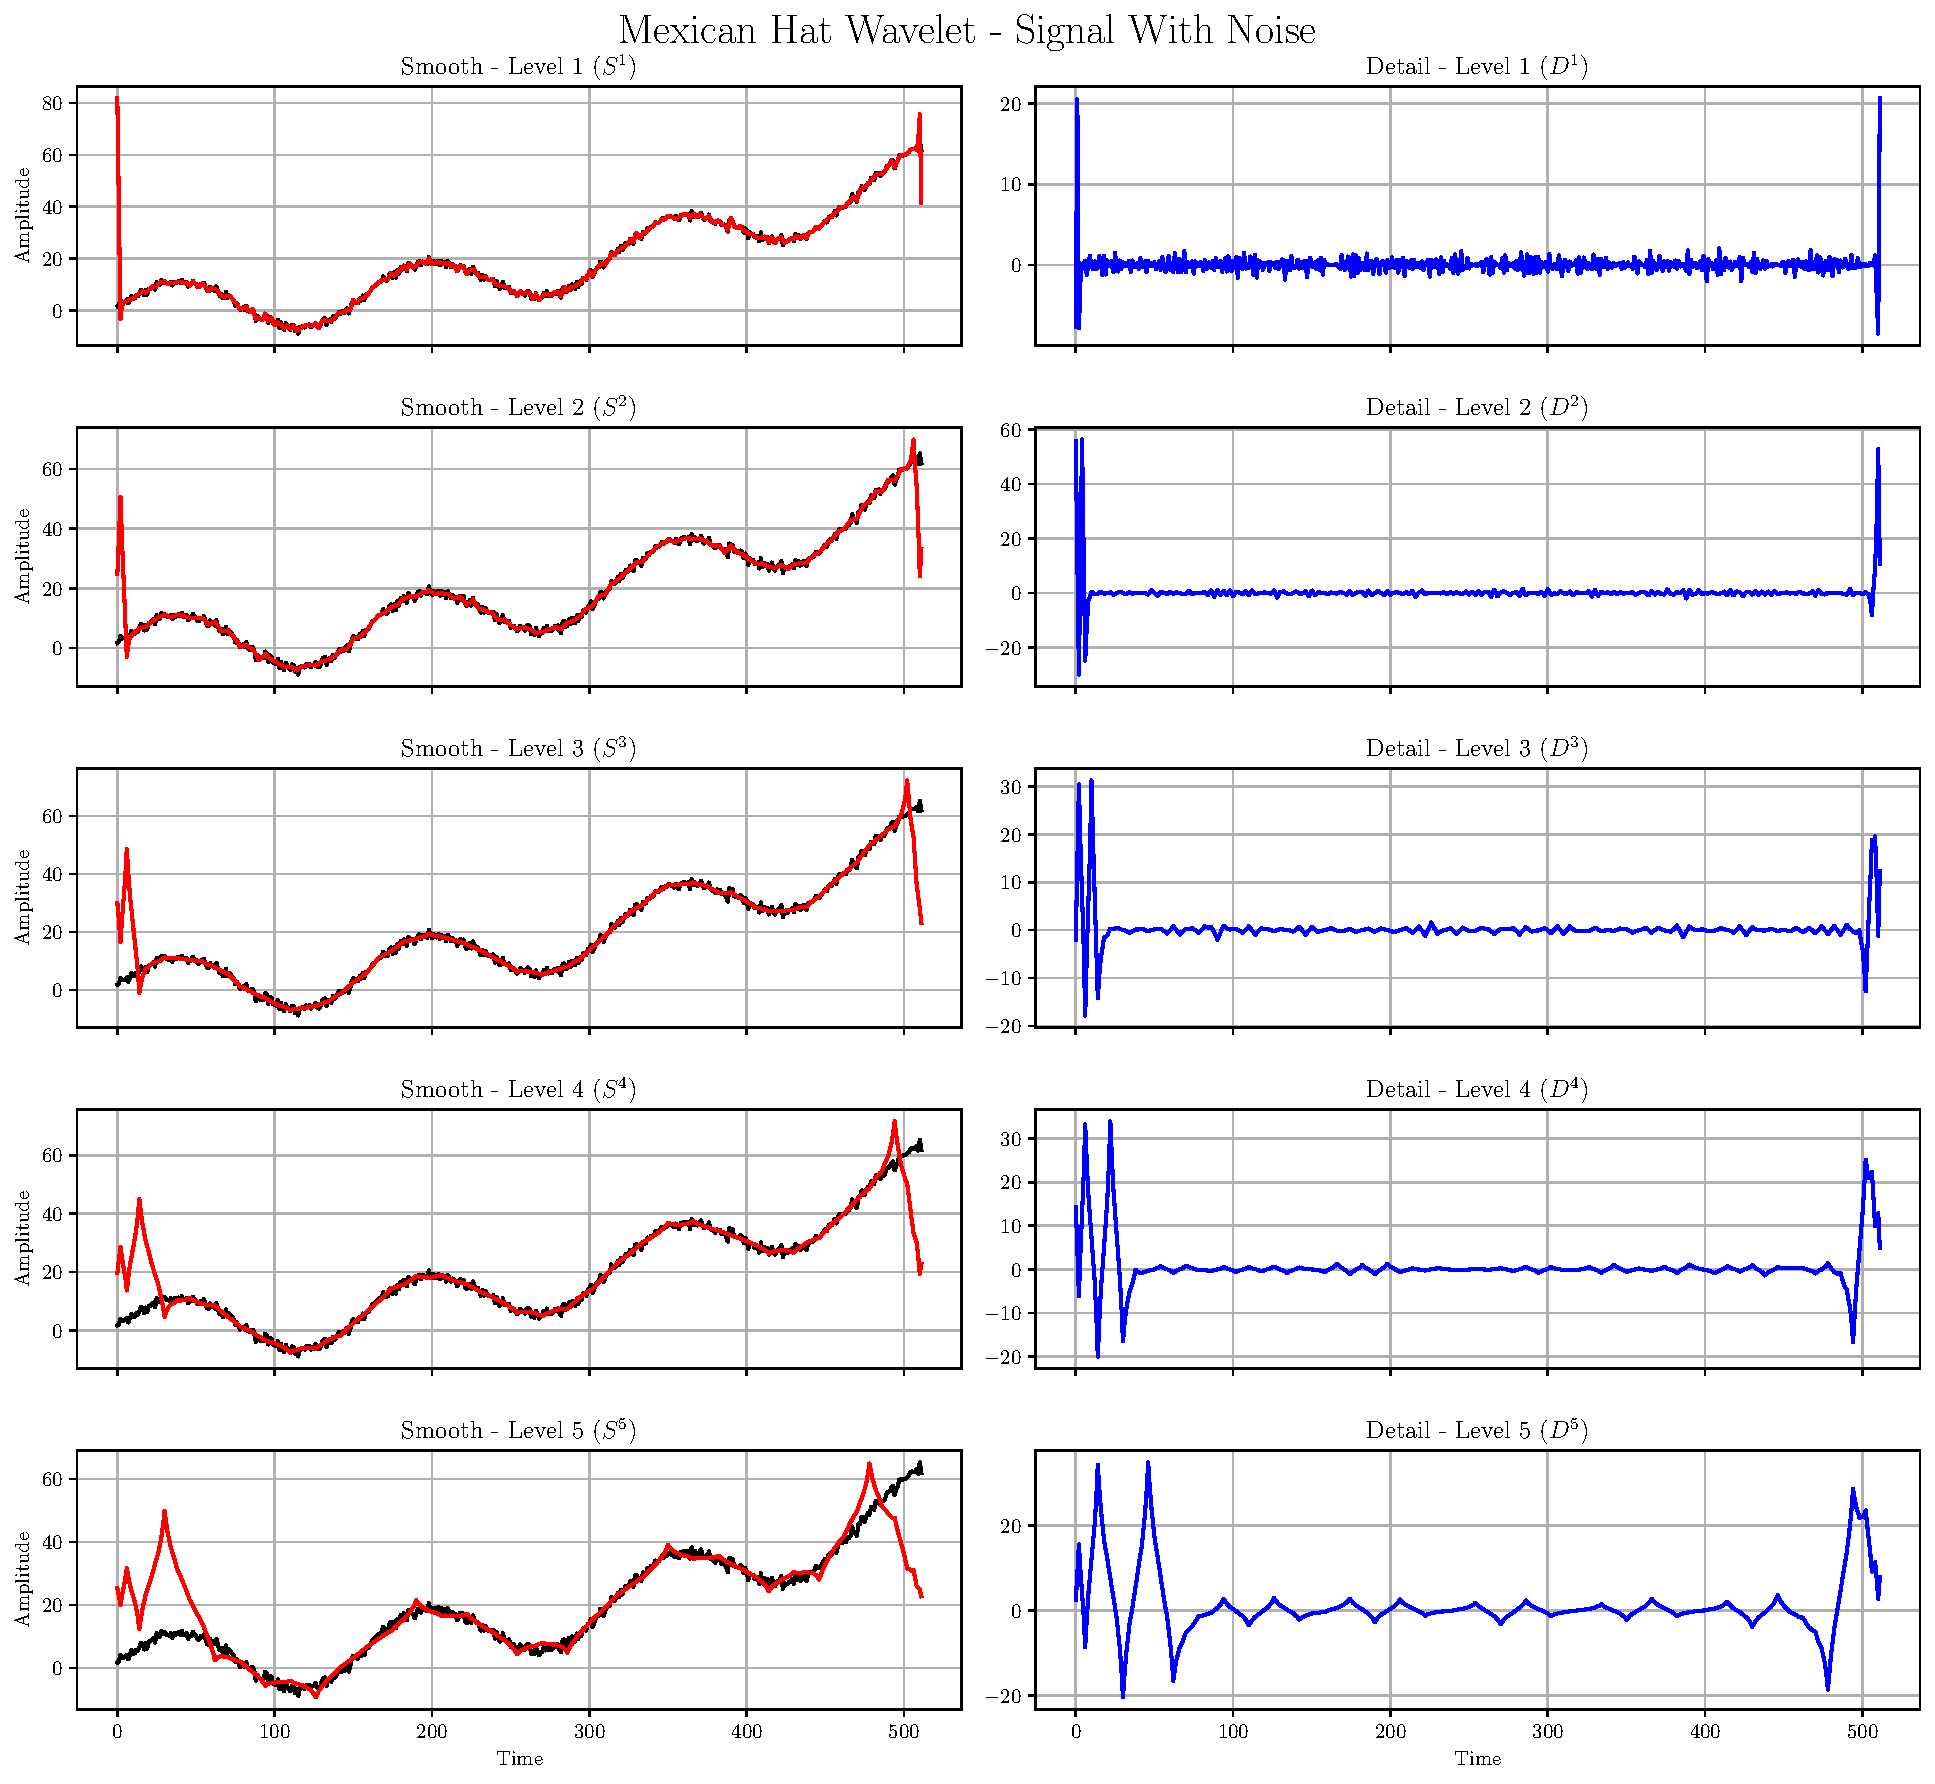
\includegraphics[height=11cm]{../Tests/Outputs/MexicanHatWavelet_SignalWithNoise.pdf}
		\caption{Results of Mexican Hat wavelet on the simulated signal.}
		\label{fig:1d_mh}
	\end{figure}	
	
	\clearpage
	\begin{figure}[!h]
		\centering
		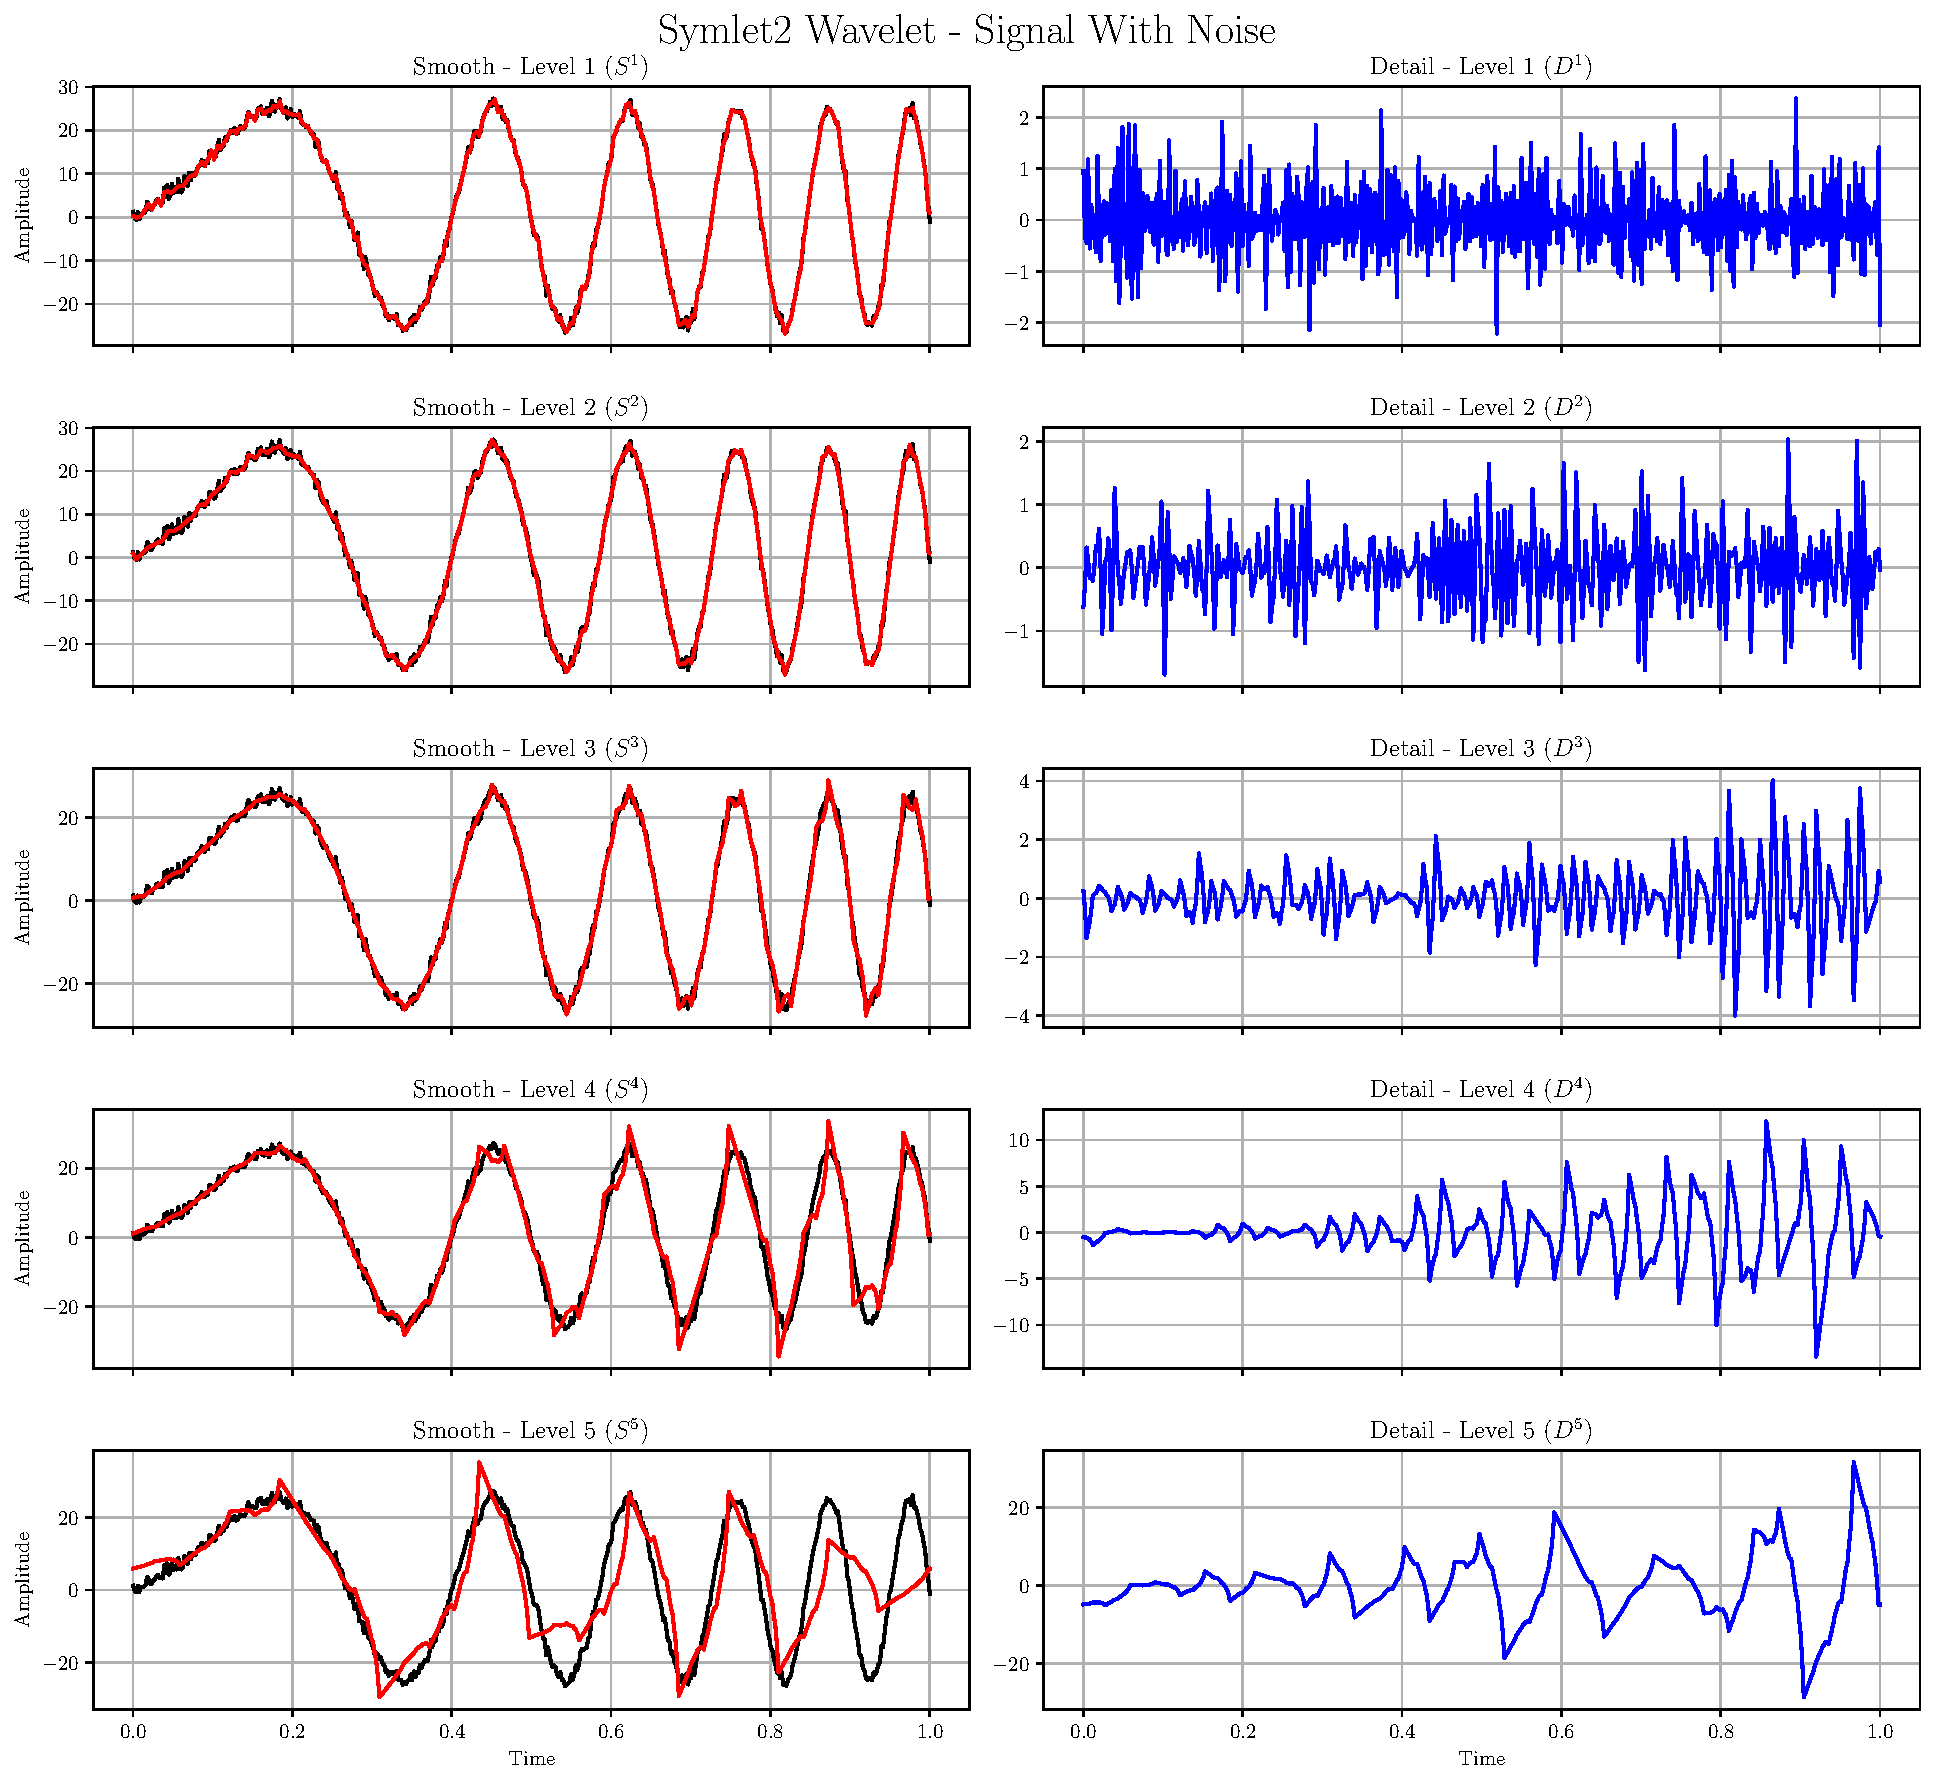
\includegraphics[height=11cm]{../Tests/Outputs/Symlet2Wavelet_SignalWithNoise.pdf}
		\caption{Results of Symlet2 wavelet on the simulated signal.}
		\label{fig:1d_sym2}
	\end{figure}
	
	For checking the results of each wavelets used, difference between the main signal is calculated from the equation \ref{eq:error}.
	
	\begin{equation}
		e^k = \|f-S^k\|_2
		\label{eq:error}
	\end{equation}
	
	\begin{table}[h!]
		\centering
		\caption{Error for used wavelets.}
		\vspace{0.3cm}
		\renewcommand{\arraystretch}{1.4}
		\begin{tabular}{c|c|c|c|c|c}
			\textbf{Level} & \textbf{Haar} & \textbf{Daubechies4} & \textbf{Daubechies6} & \textbf{Mexican Hat} & \textbf{Symlet2} \\
			\hline 
			1 & \textcolor{blue}{22.3967} & 16.1461 & 15.9328 & 16.2191 & 14.7038 \\
			2 & 35.8193 & \textcolor{blue}{12.1606} & \textcolor{green}{10.8583} & \textcolor{blue}{12.2734} & \textcolor{blue}{11.8964} \\
			3 & 69.8424 & 23.5287 & 11.0108 & 22.1990 & 22.4478 \\
			4 & 135.3934 & 80.7993 & 49.7569 & 74.2519 & 73.6403 \\
			5 & 267.9761 & 202.0768 & 146.3352 & 159.4626 & 201.1597 \\
		\end{tabular}
		\label{tab:errors}
	\end{table}
	
	As shown in the table \ref{tab:errors}, best result was achieved with level 2 of Daubechies6 Wavelet.
	
	\subsubsection{GNSS Signal Cycle Slip Detection}
	
	The studied signal is for GPS PRN03 which is shown in the figure \ref{fig:GPS_Signal}. This signal contains two cycle slips occurred in indices of 119 and 374 (times are 5.9583 and 7.2500 hour of day). Results for 5 mentioned wavelets are shown in the figures \ref{fig:cs_haar} to \ref{fig:cs_sym2}. 
	
	\begin{figure}[!h]
		\centering
		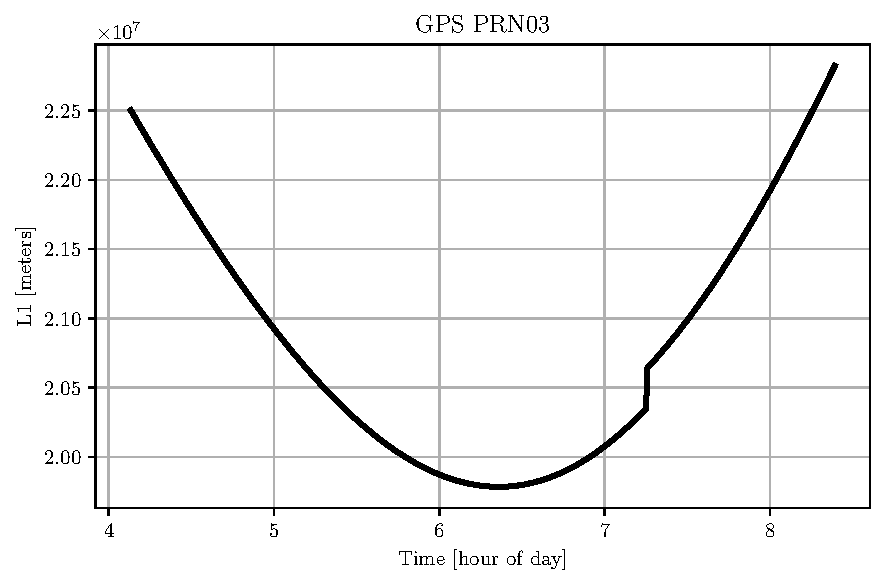
\includegraphics[height=7cm]{../Tests/Outputs/CycleSlip_MainSignal.pdf}
		\caption{GPS signal with cycle slip.}
		\label{fig:GPS_Signal}
	\end{figure}
	
	\begin{figure}[!h]
		\centering
		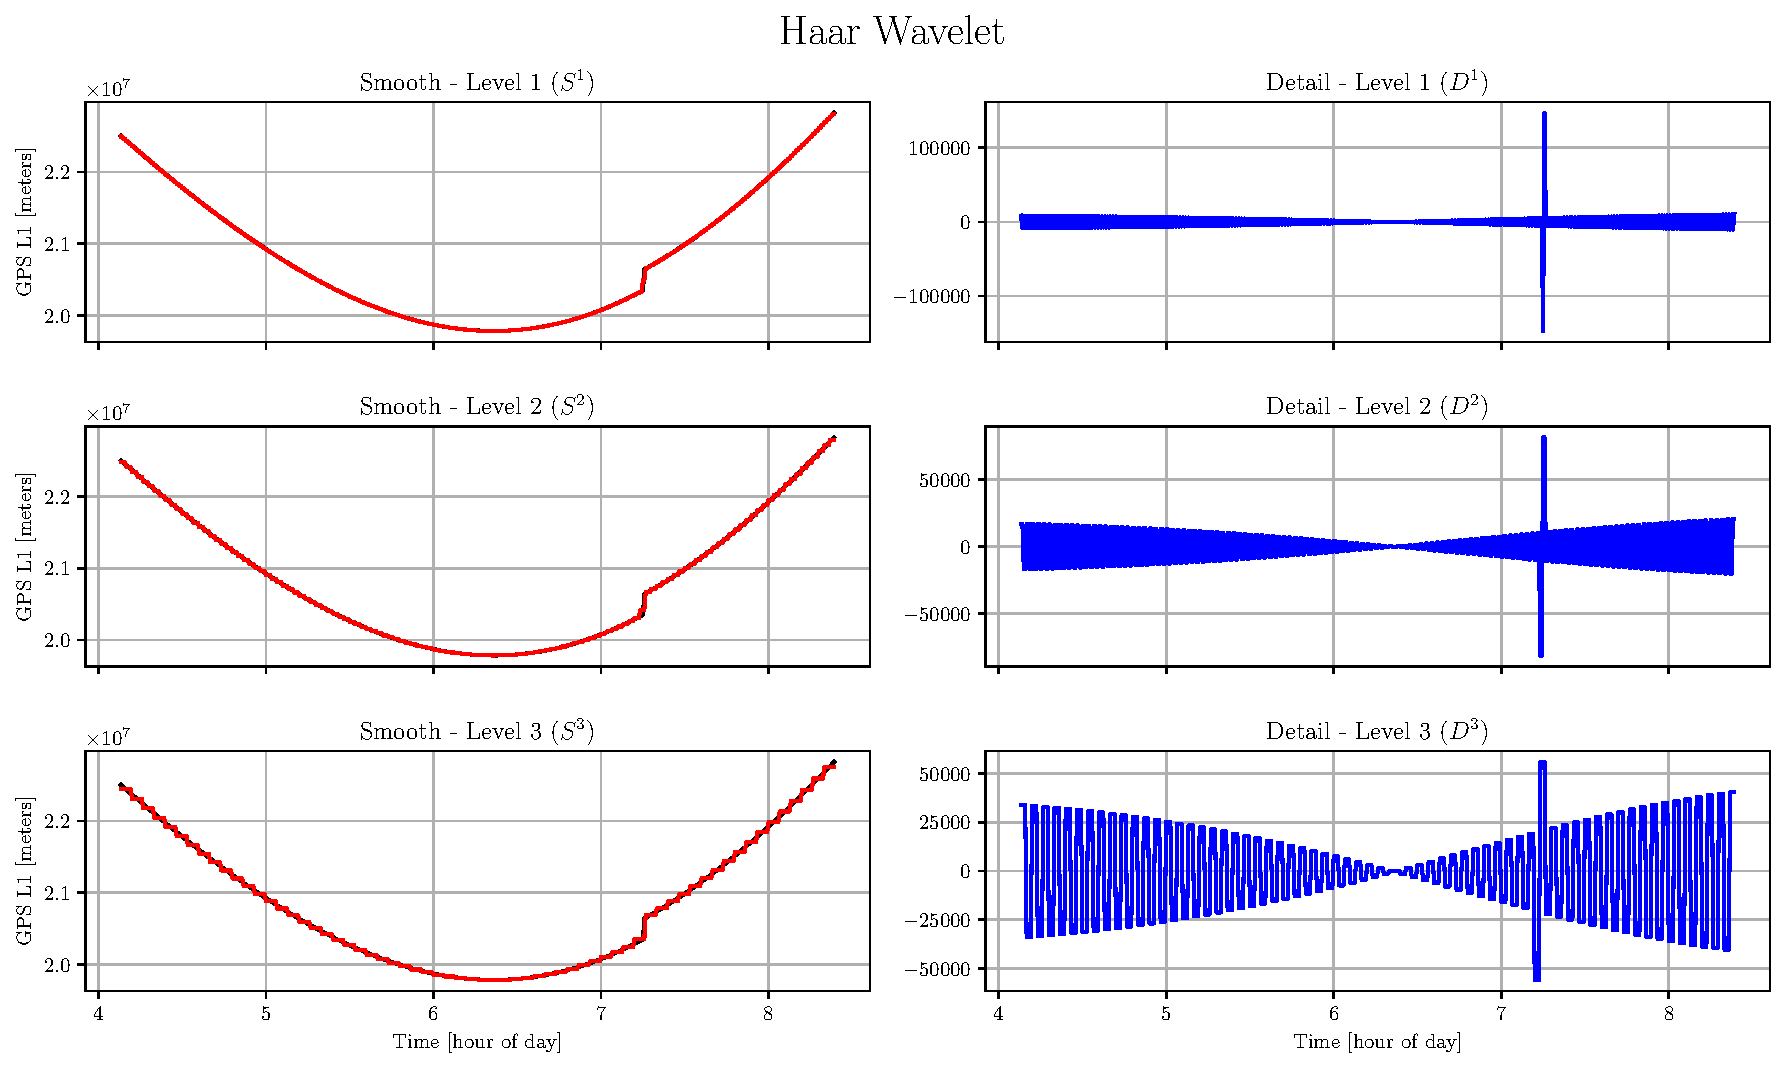
\includegraphics[height=7cm]{../Tests/Outputs/CycleSlip_Haar.pdf}
		\caption{Results of Haar wavelet on GPS signal.}
		\label{fig:cs_haar}
	\end{figure}
	
	\begin{figure}[!h]
		\centering
		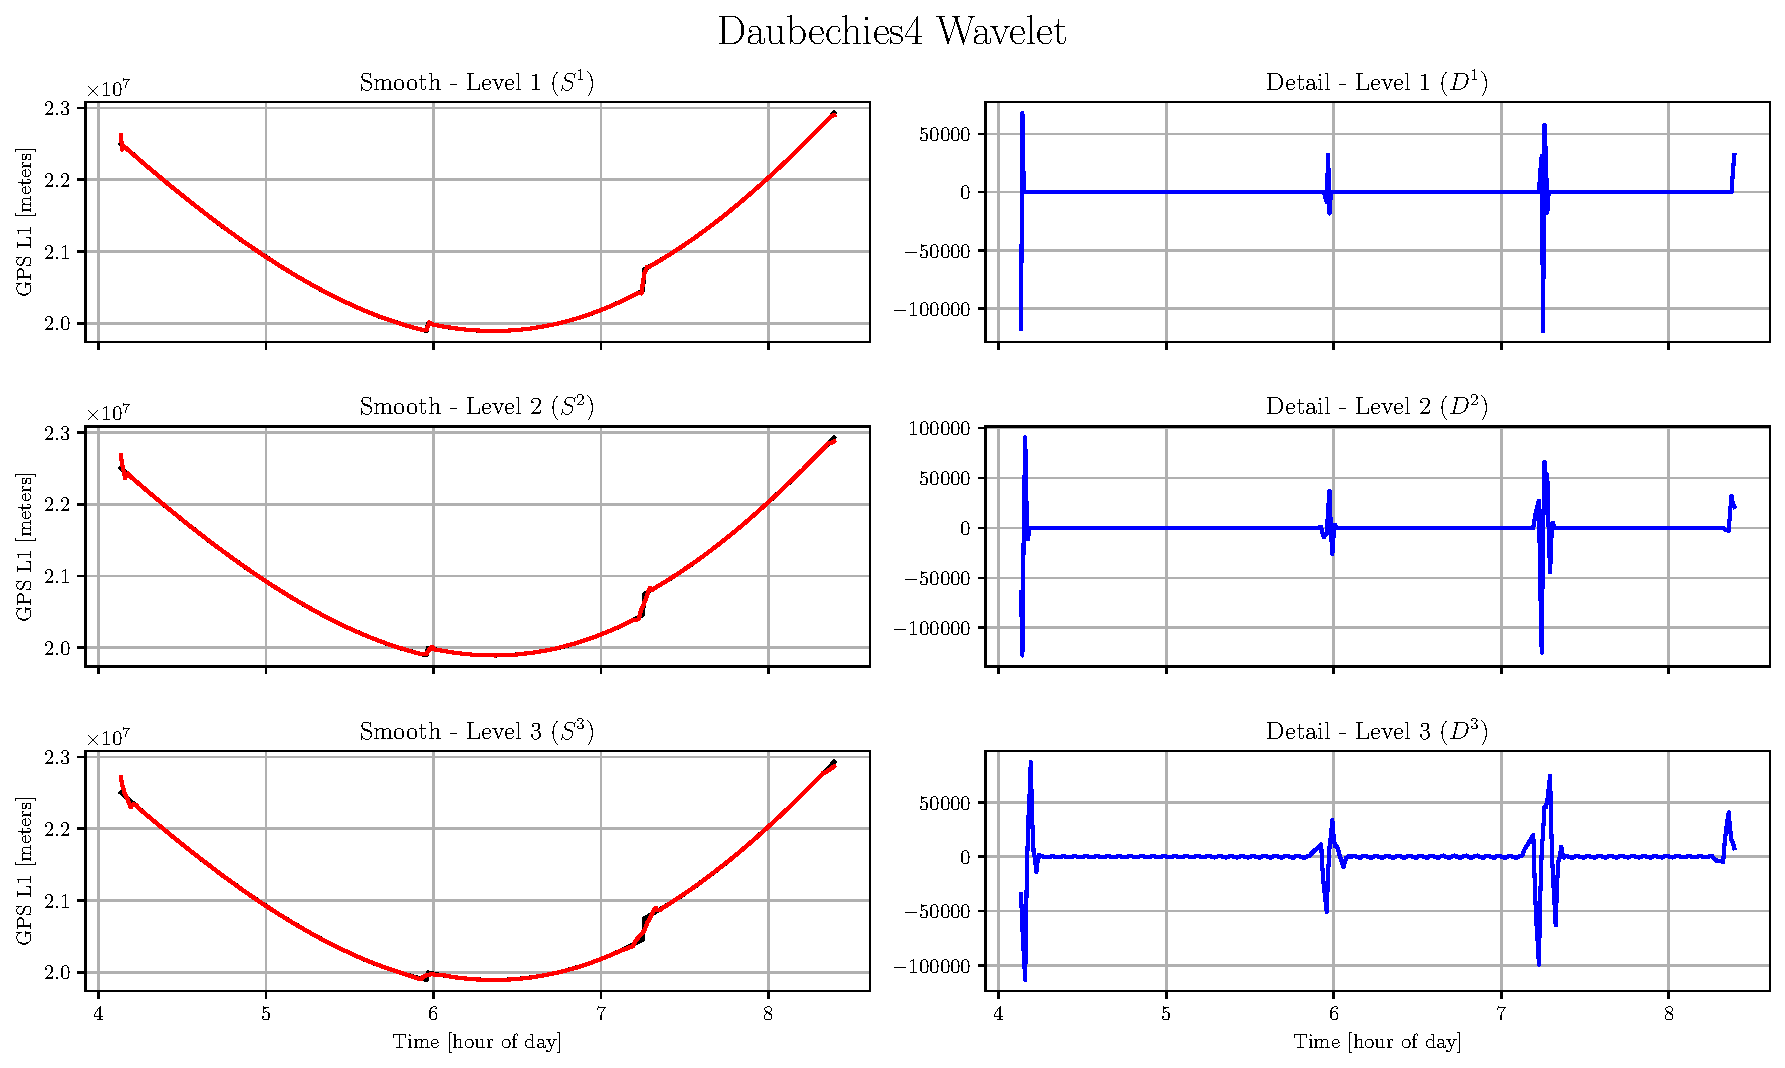
\includegraphics[height=7cm]{../Tests/Outputs/CycleSlip_Daubechies4.pdf}
		\caption{Results of Daubechies4 wavelet on GPS signal.}
		\label{fig:cs_db4}
	\end{figure}
	
	\begin{figure}[!h]
		\centering
		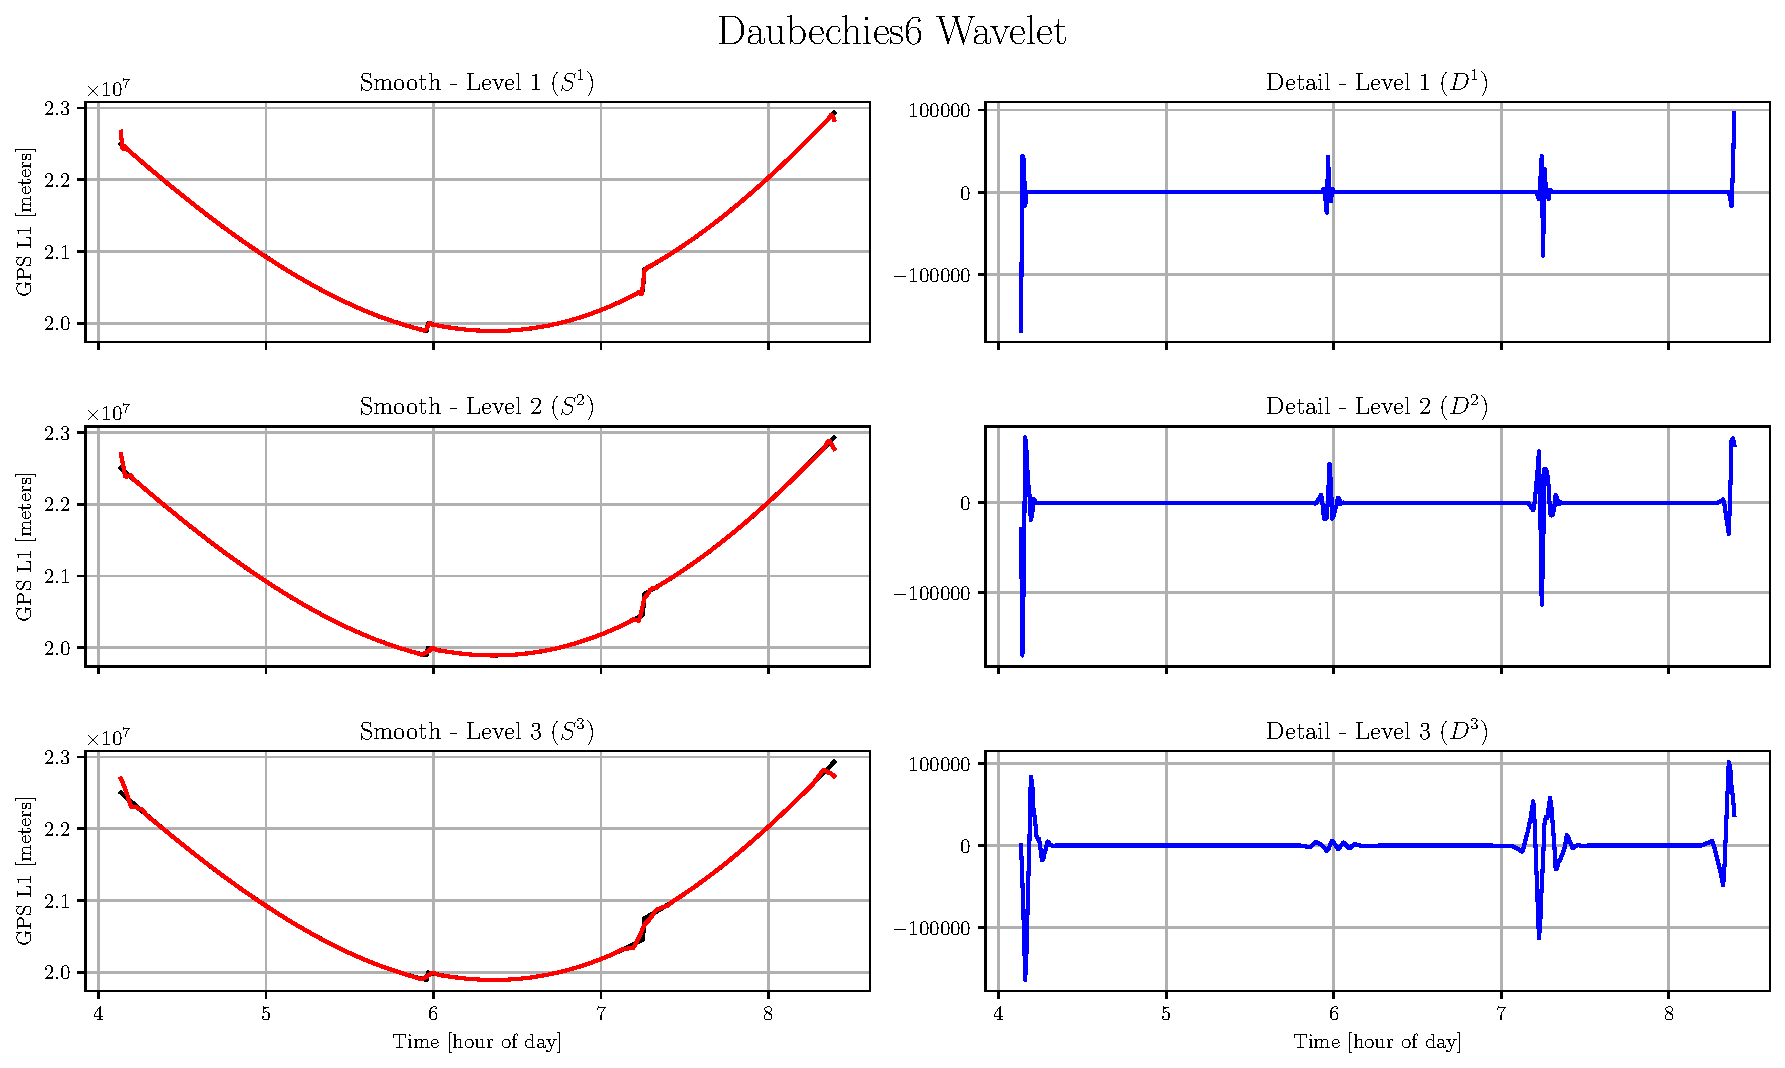
\includegraphics[height=7cm]{../Tests/Outputs/CycleSlip_Daubechies6.pdf}
		\caption{Results of Daubechies6 wavelet on GPS signal.}
		\label{fig:cs_db6}
	\end{figure}
	
	\begin{figure}[!h]
		\centering
		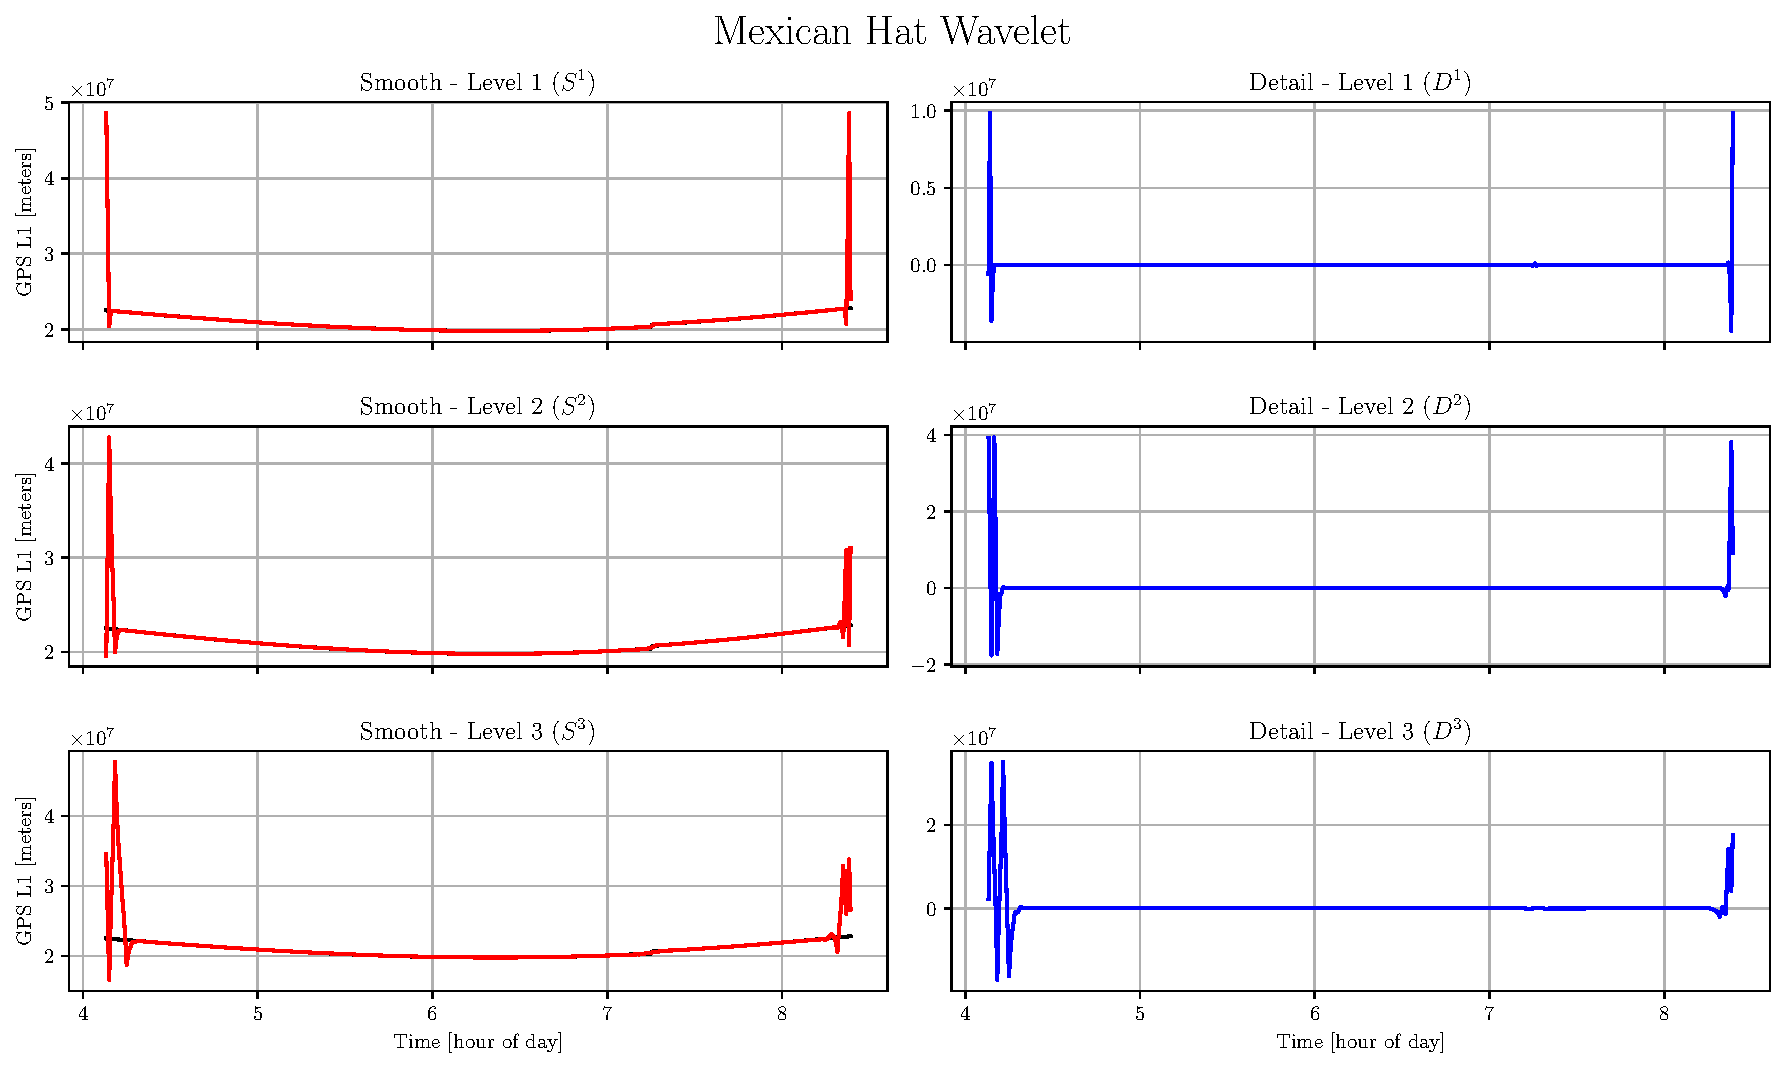
\includegraphics[height=7cm]{../Tests/Outputs/CycleSlip_MexicanHat.pdf}
		\caption{Results of Mexican Hat wavelet on GPS signal.}
		\label{fig:cs_mh}
	\end{figure}
	
	\begin{figure}[!h]
		\centering
		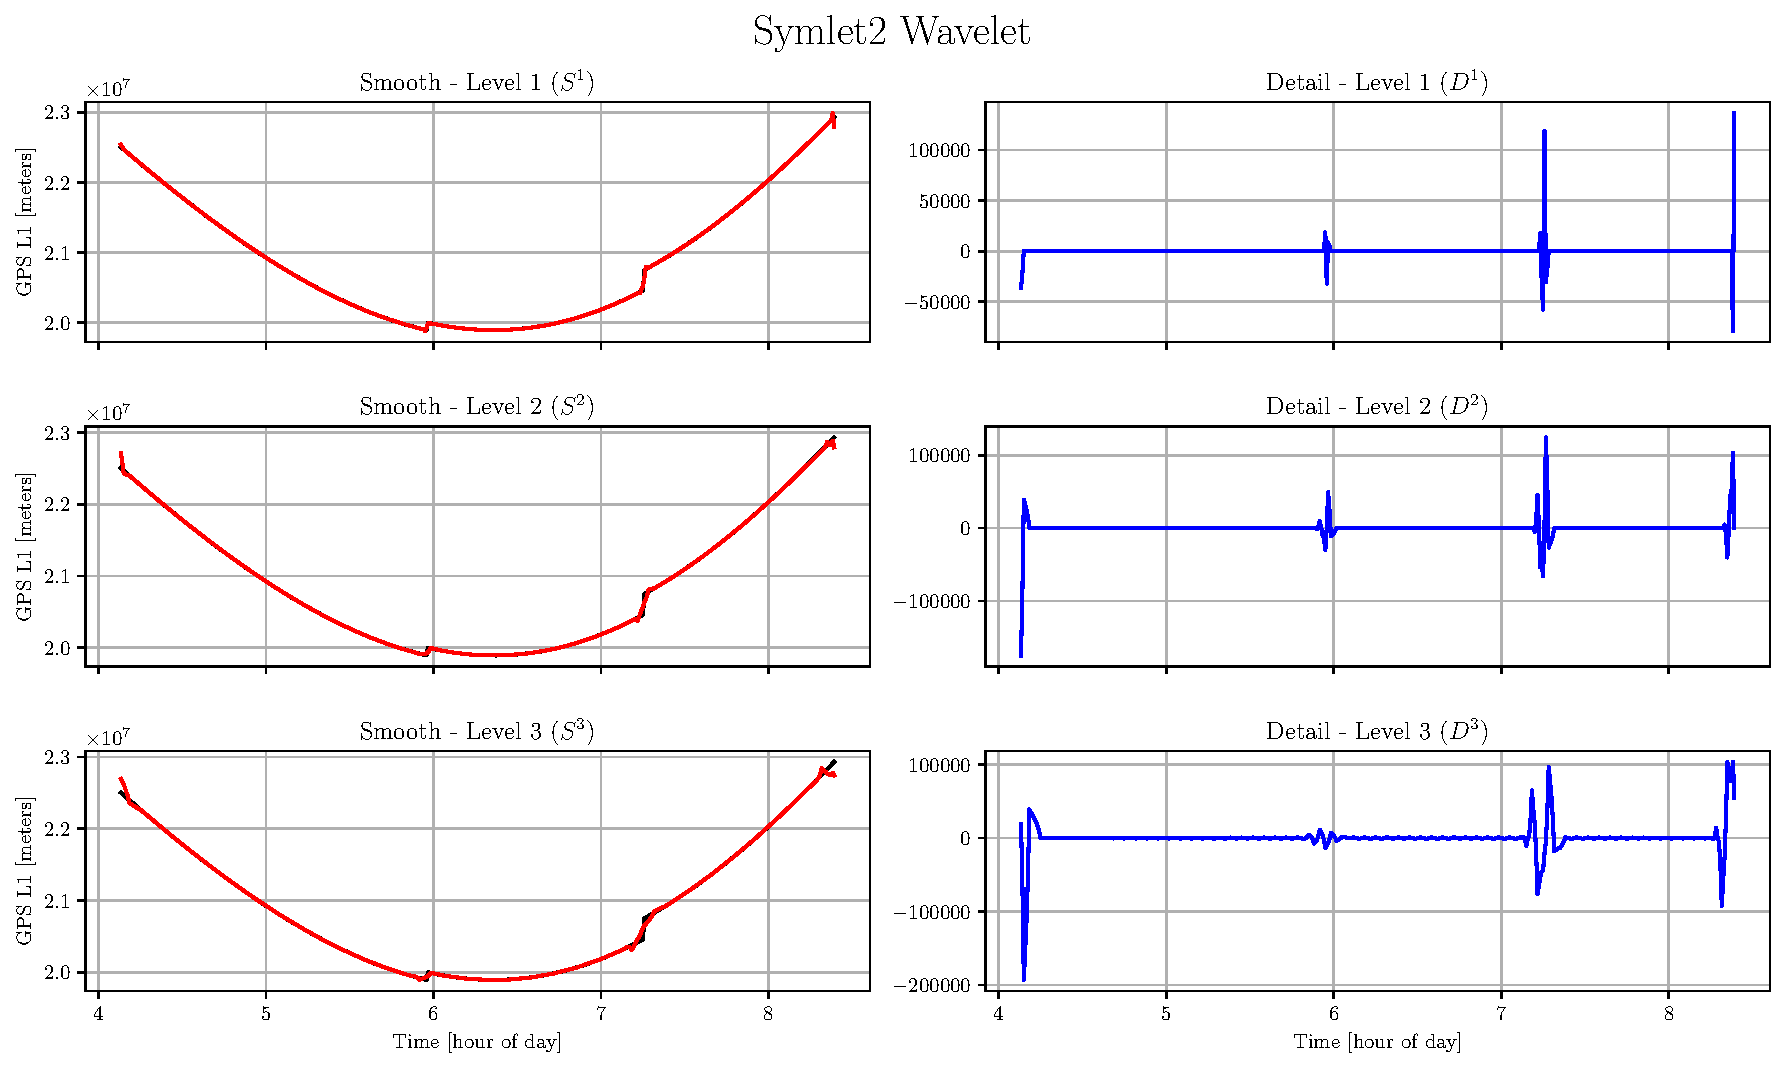
\includegraphics[height=7cm]{../Tests/Outputs/CycleSlip_Symlet2.pdf}
		\caption{Results of Symlet2 wavelet on GPS signal.}
		\label{fig:cs_sym2}
	\end{figure}
	\clearpage
	
	As can be seen from the figures, the first cycle slip, which is smaller in magnitude, is not detectable in the Haar details of levels 1 and 2, but it can be detected in the other four wavelets. To determine the timing of occurred cycle slips from the detail components, a 3-sigma test was applied using equation \ref{eq:CycleSlip_idx}. Values falling within this range were identified as cycle slips. Results are shown in the table \ref{tab:CycleSlips}.
	
	\begin{equation}
		\begin{gathered}
			cs > \mu_D + 3\sigma_D^2 \\
			cs < \mu_D - 3\sigma_D^2
		\end{gathered}
		\label{eq:CycleSlip_idx}
	\end{equation}
	
	\begin{table}[h!]
		\centering
		\caption{Detected cycle slips from implemented wavelets.}
		\vspace{0.3cm}
		\renewcommand{\arraystretch}{1.4}
		\begin{tabular}{c|c|c}
			\textbf{Wavelet} & \textbf{Indices} & \textbf{Times (hour of day)} \\
			\hline 
			\text{Haar} & \text{374, 375} & \text{7.25, 7.26} \\
			\text{Daubechies4} & \text{220, 373, 374, 375, 375, 376} & \text{5.97, 7.24, 7.25, 7.26, 7.27} \\
			\text{Daubechies6} & \text{219, 220, 373, 374, 375} & \text{5.96, 5.97, 7.24, 7.25, 7.26} \\
			\text{Mexican Hat} & \text{219, 373, 374, 375, 376} & \text{5.96, 7.24, 7.25, 7.26, 7.27} \\
			\text{Symlet2} & \text{219, 373, 374, 375, 376} & \text{5.96, 7.24, 7.25, 7.26, 7.27} \\
		\end{tabular}
		\label{tab:CycleSlips}
	\end{table}
	
	\subsection{Two-Dimensional}
	
	The studied Image is shown in figure \ref{fig:2d_image}. Two types of noise are added to this image (salt\&pepper and Gaussian). Results for different types of wavelets are shown in the figures \ref{fig:2d_haar} to \ref{fig:2d_sym2_gs}
	
	\begin{figure}[!h]
		\centering
		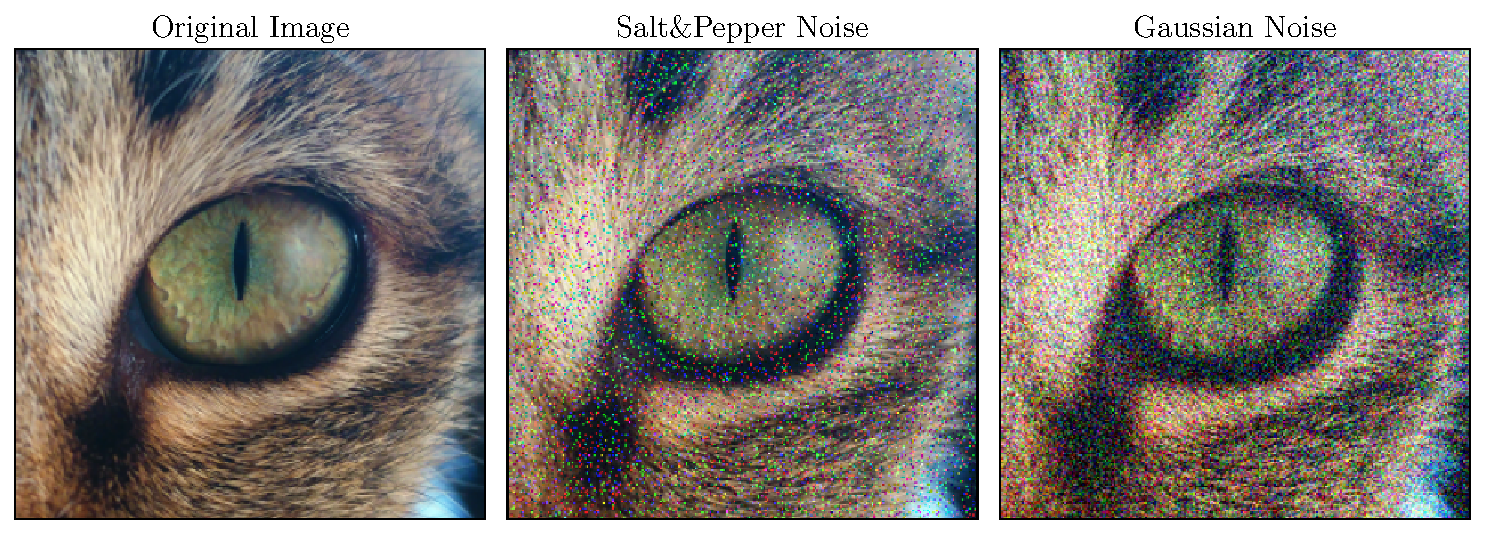
\includegraphics[height=5.5cm]{../Tests/Outputs/2D_Image.pdf}
		\caption{Original image alongside noisy images.}
		\label{fig:2d_image}
	\end{figure}

	% Haar
	\begin{figure}[!h]
		\centering
		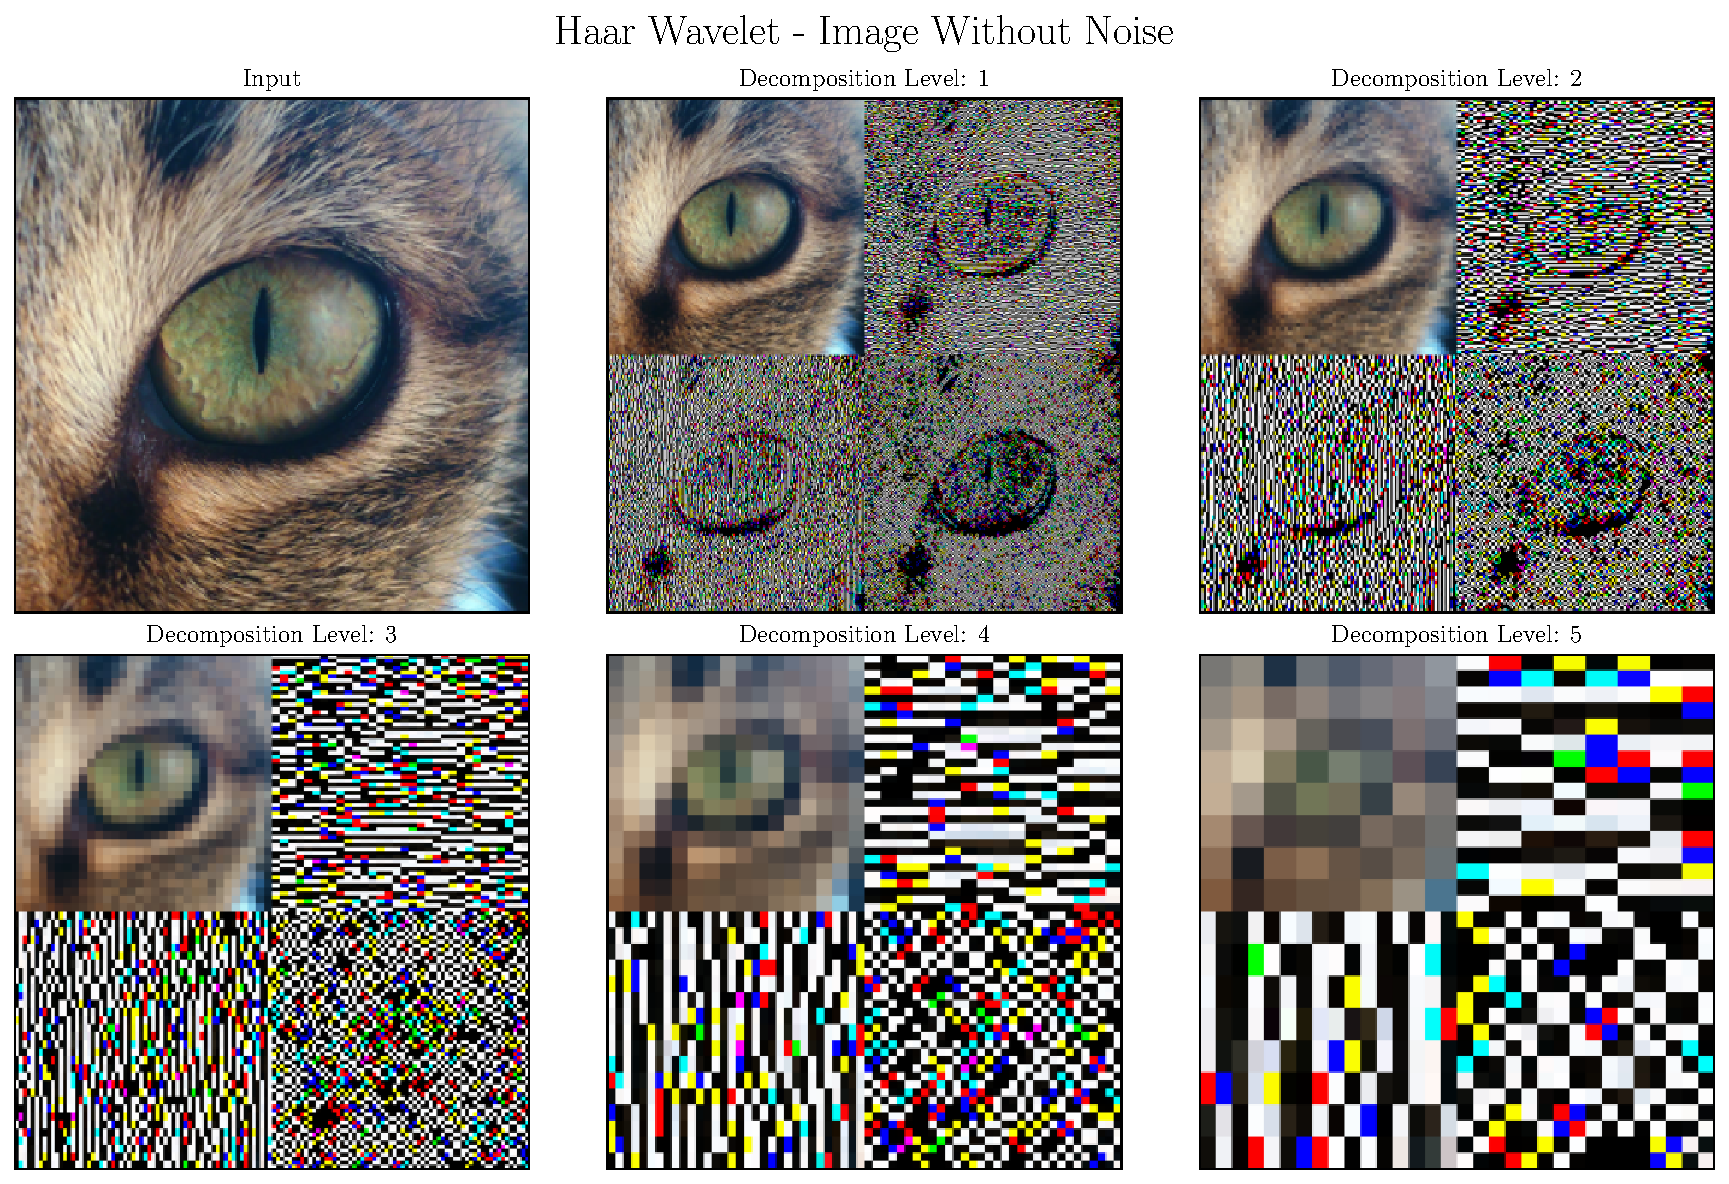
\includegraphics[height=7cm]{../Tests/Outputs/2D_HaarWavelet_WithoutNoise.pdf}
		\caption{Results of Haar wavelet on original image.}
		\label{fig:2d_haar}
	\end{figure}

	\begin{figure}[!h]
		\centering
		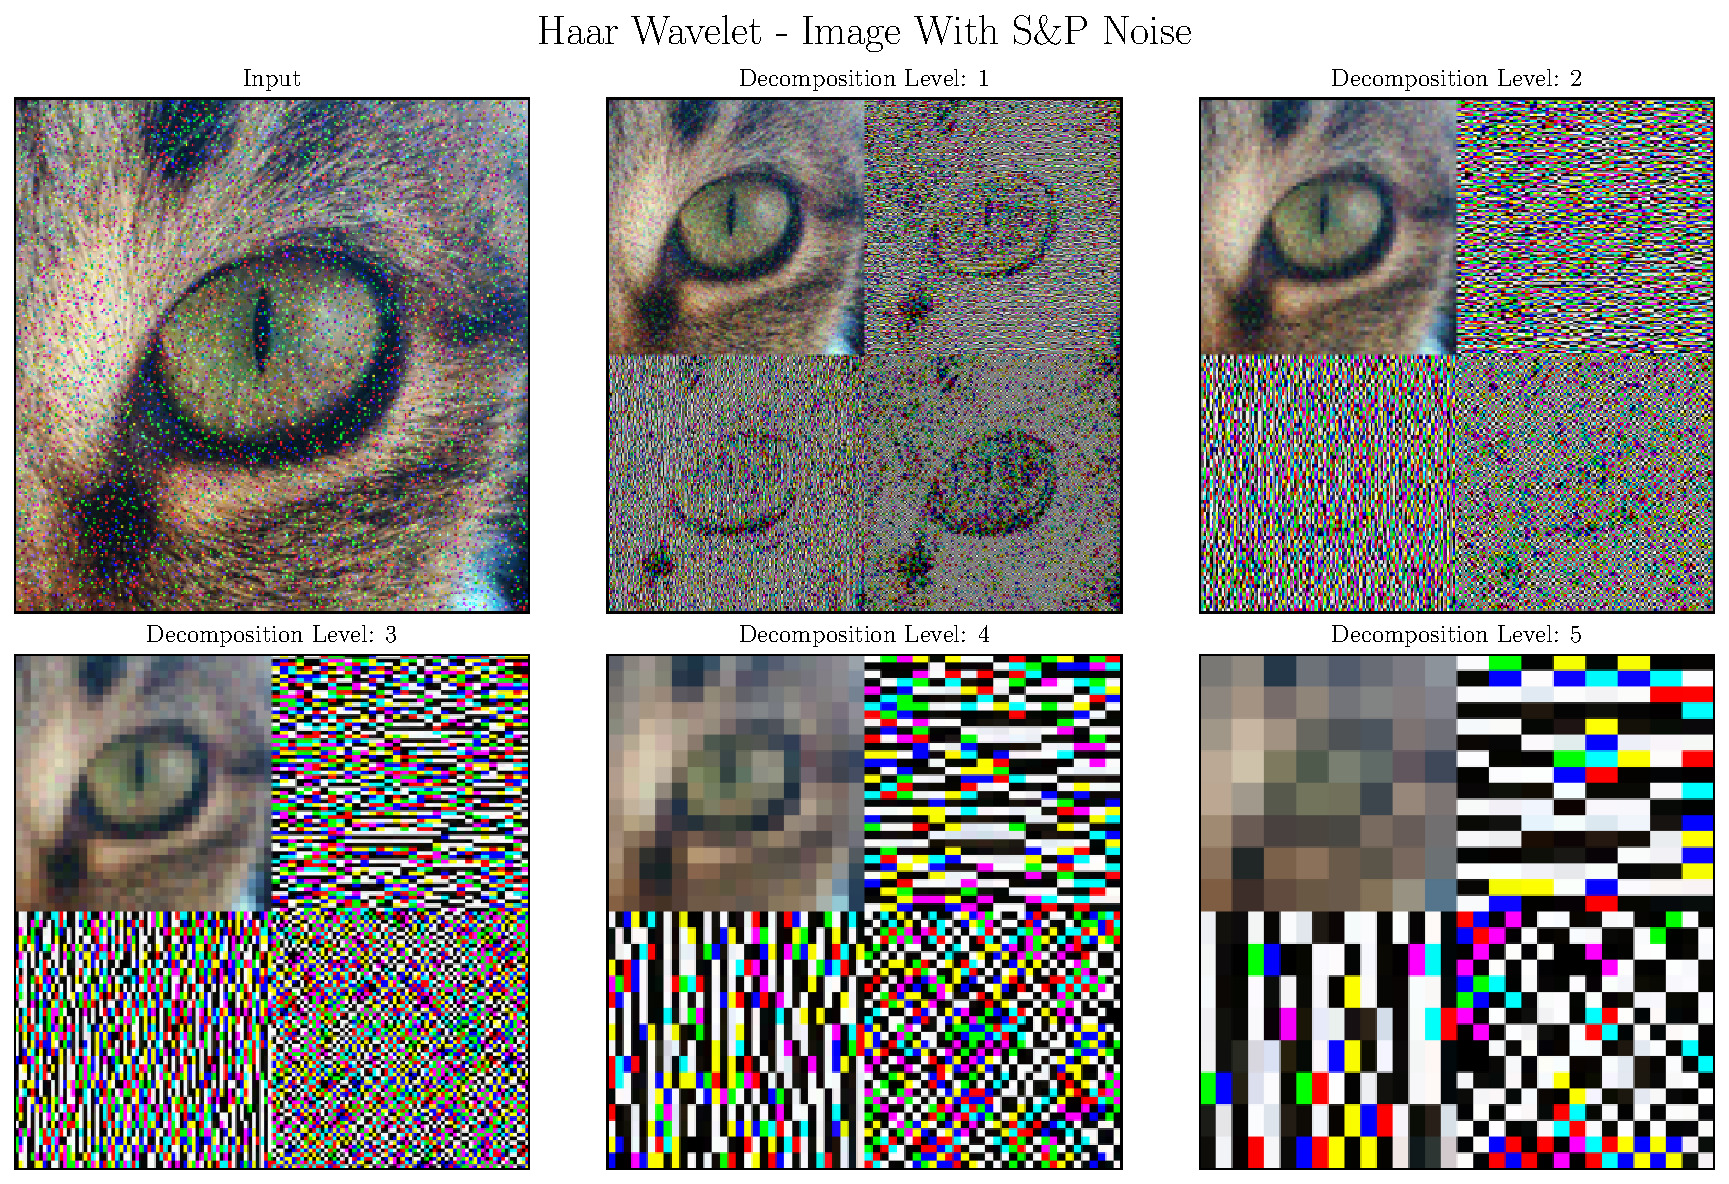
\includegraphics[height=7cm]{../Tests/Outputs/2D_HaarWavelet_SPNoise.pdf}
		\caption{Results of Haar wavelet on image with s\&p noise.}
		\label{fig:2d_haar_sp}
	\end{figure}
	
	\begin{figure}[!h]
		\centering
		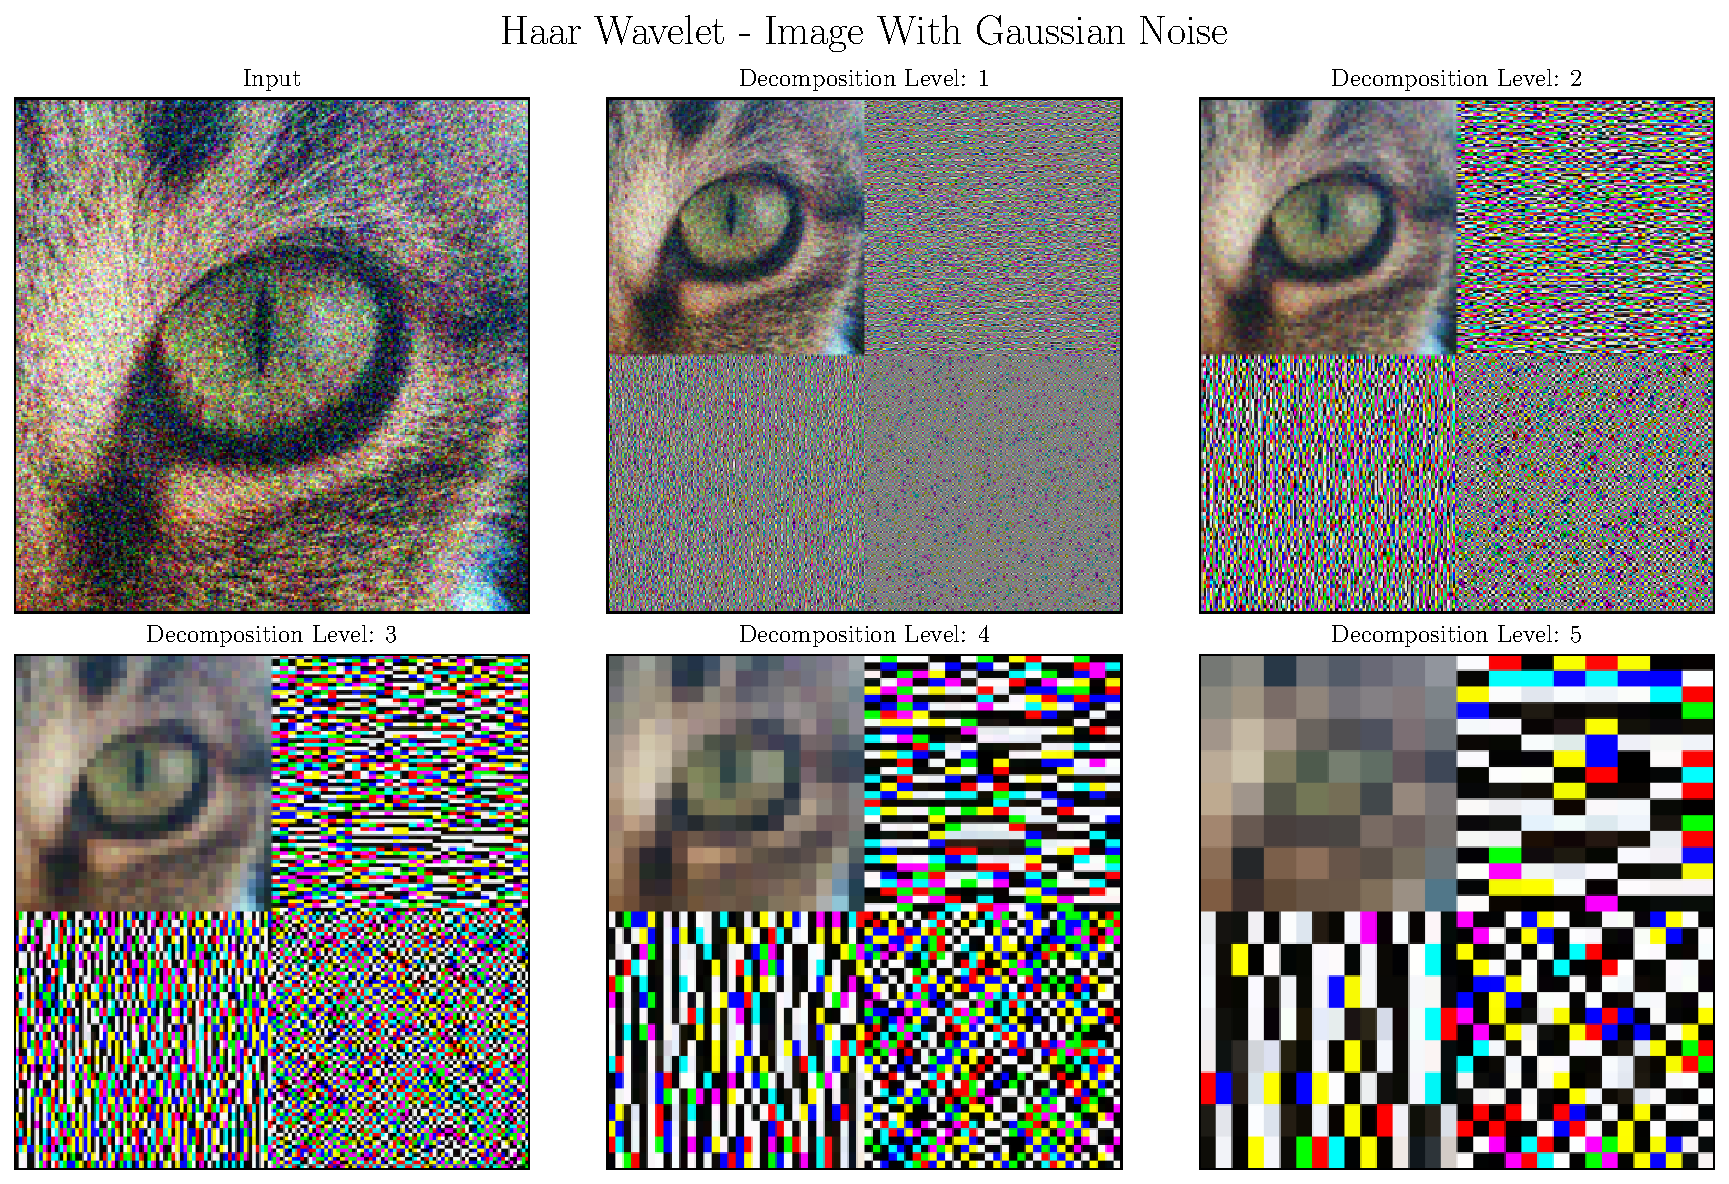
\includegraphics[height=7cm]{../Tests/Outputs/2D_HaarWavelet_GaussianNoise.pdf}
		\caption{Results of Haar wavelet on image with Gaussian noise.}
		\label{fig:2d_haar_gs}
	\end{figure}
	
	% Daubechies4
	\begin{figure}[!h]
		\centering
		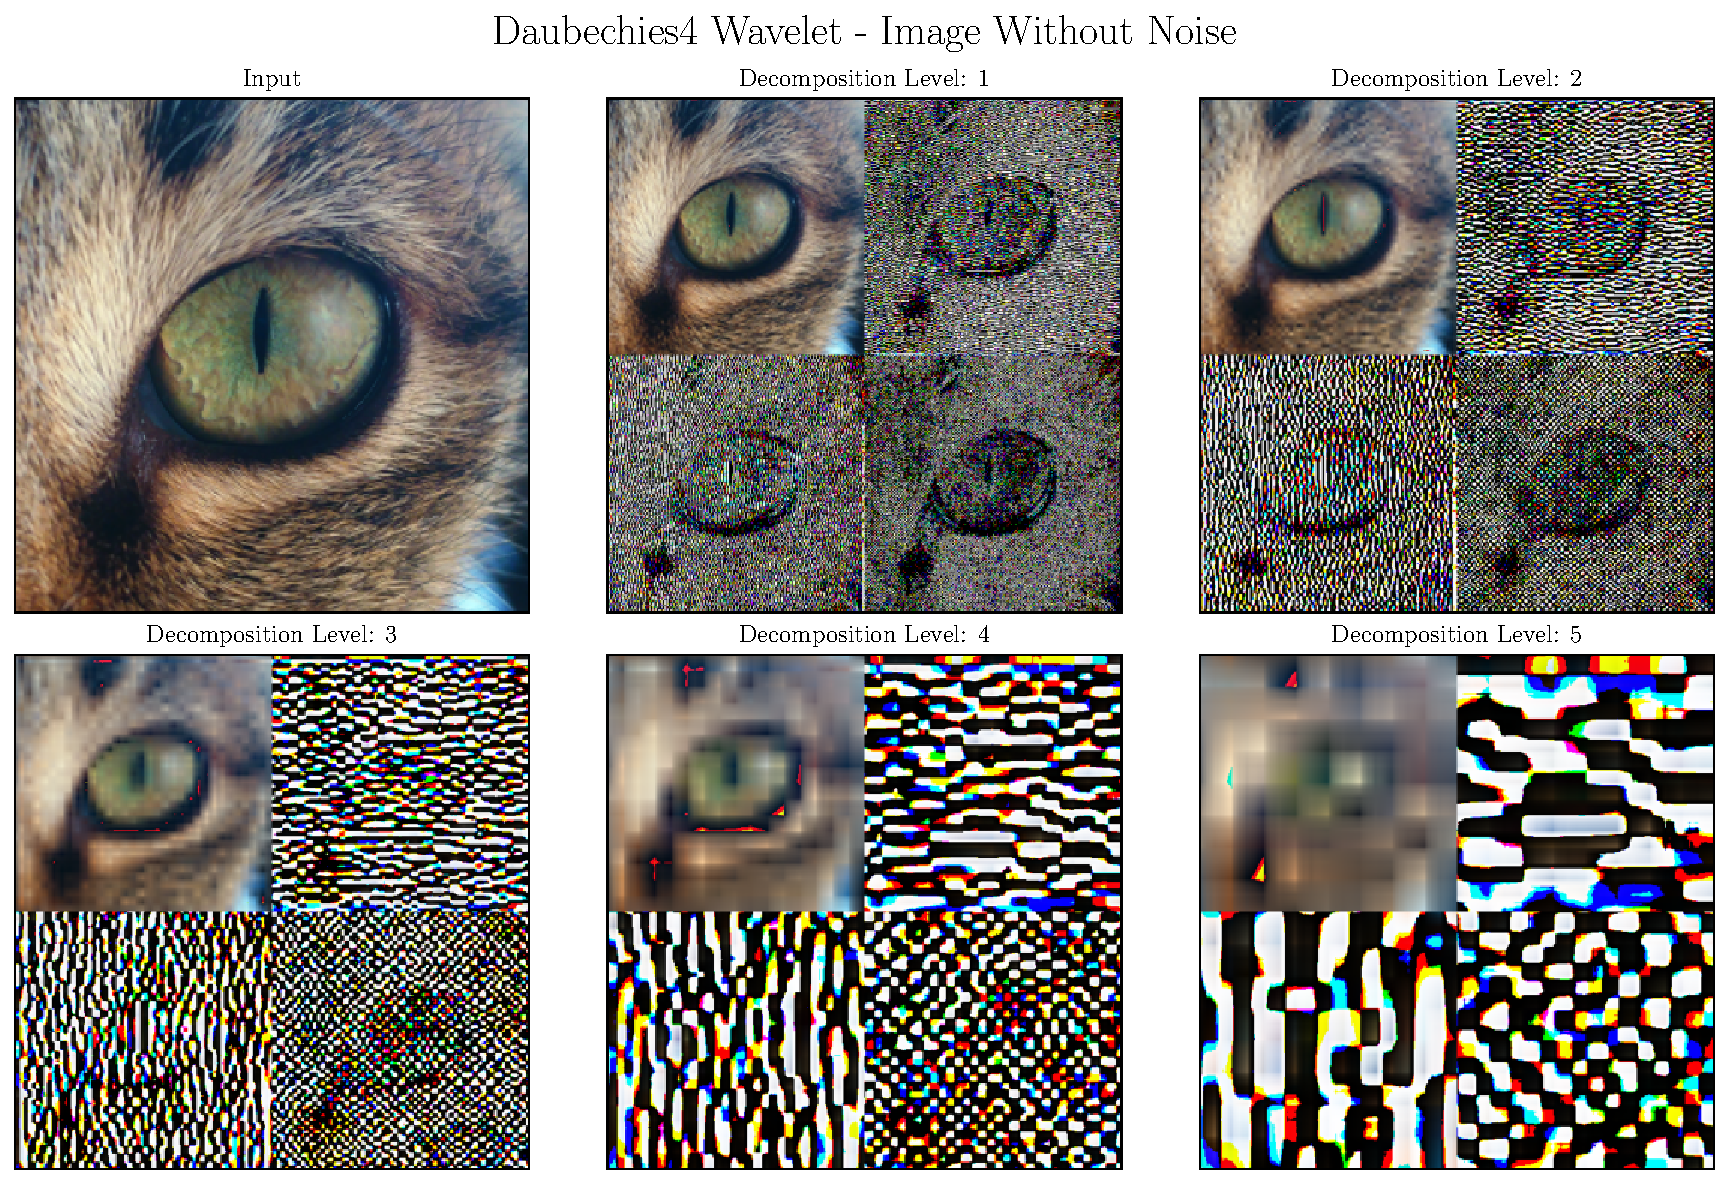
\includegraphics[height=7cm]{../Tests/Outputs/2D_Daubechies4Wavelet_WithoutNoise.pdf}
		\caption{Results of Daubechies4 wavelet on original image.}
		\label{fig:2d_db4}
	\end{figure}
	
	\begin{figure}[!h]
		\centering
		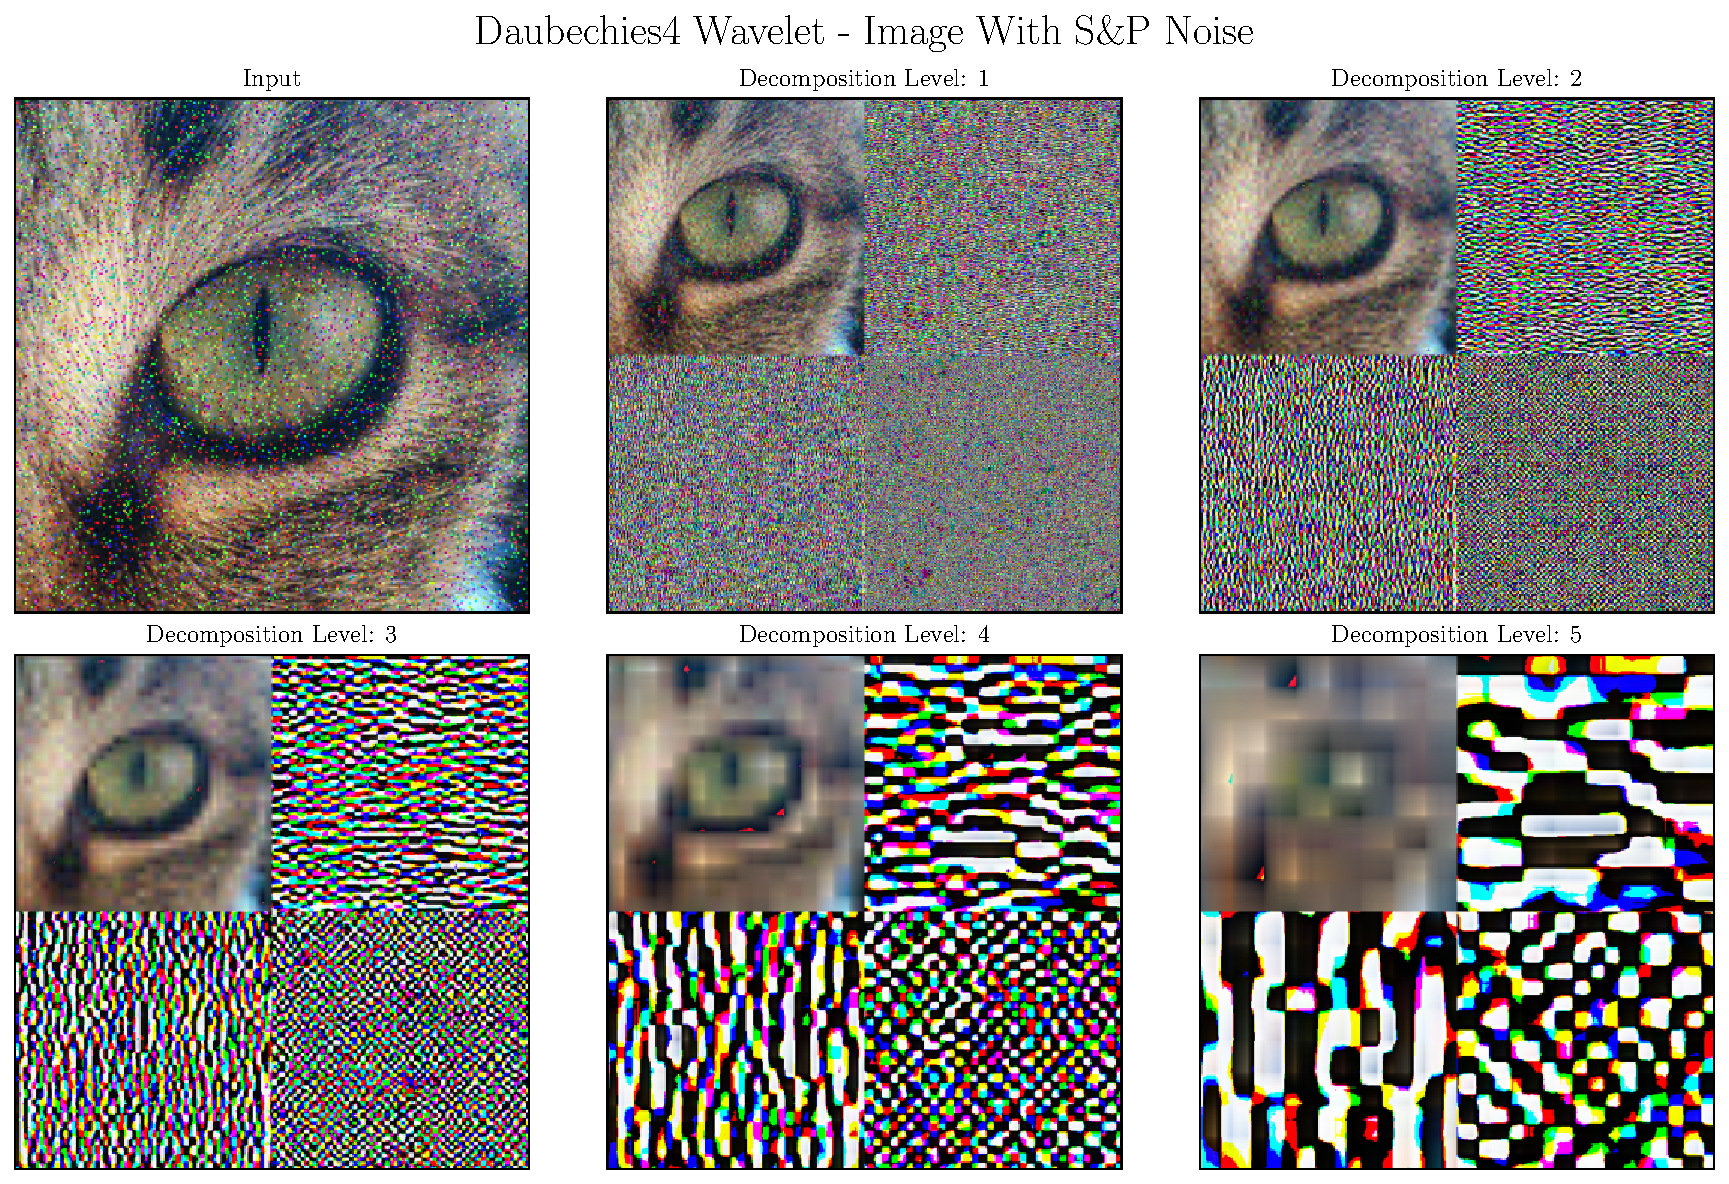
\includegraphics[height=7cm]{../Tests/Outputs/2D_Daubechies4Wavelet_SPNoise.pdf}
		\caption{Results of Daubechies4 wavelet on image with s\&p noise.}
		\label{fig:2d_db4_sp}
	\end{figure}
	
	\begin{figure}[!h]
		\centering
		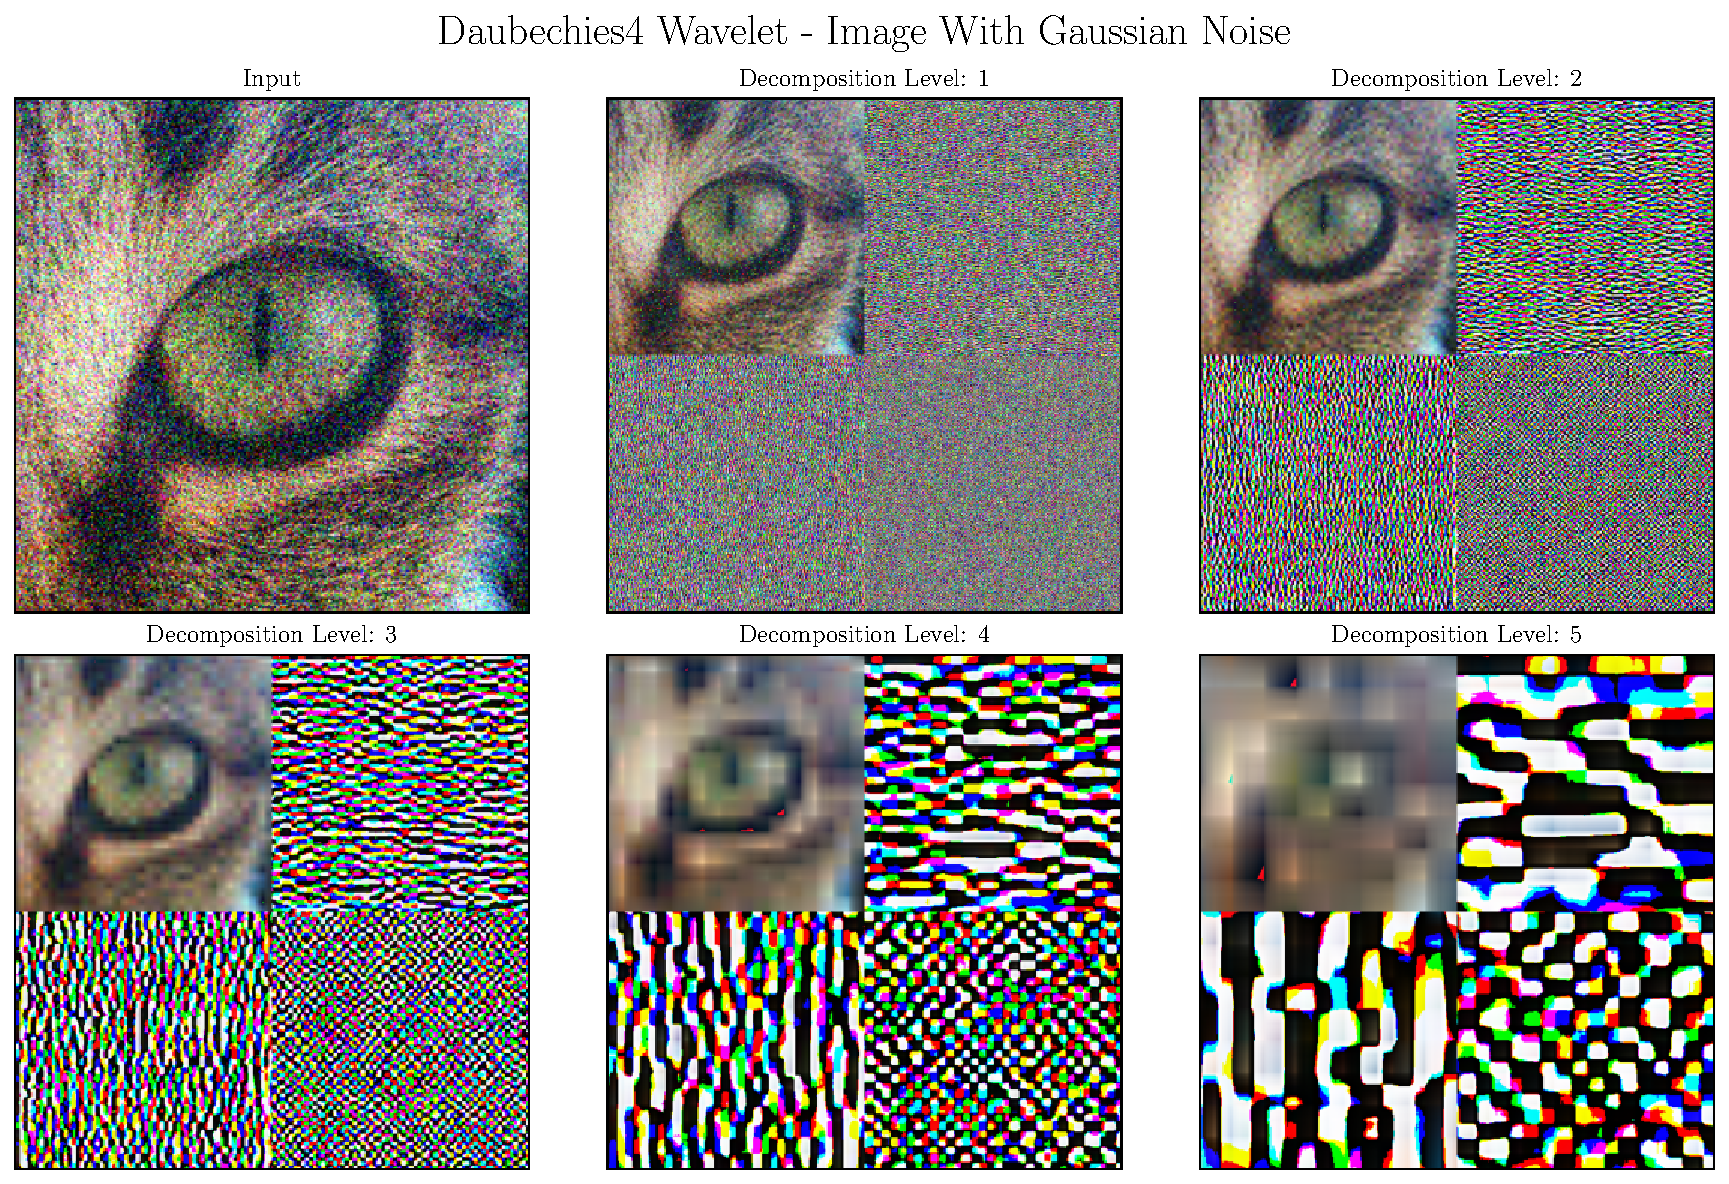
\includegraphics[height=7cm]{../Tests/Outputs/2D_Daubechies4Wavelet_GaussianNoise.pdf}
		\caption{Results of Daubechies4 wavelet on image with Gaussian noise.}
		\label{fig:2d_db4_gs}
	\end{figure}
	
	% Daubechies6
	\begin{figure}[!h]
		\centering
		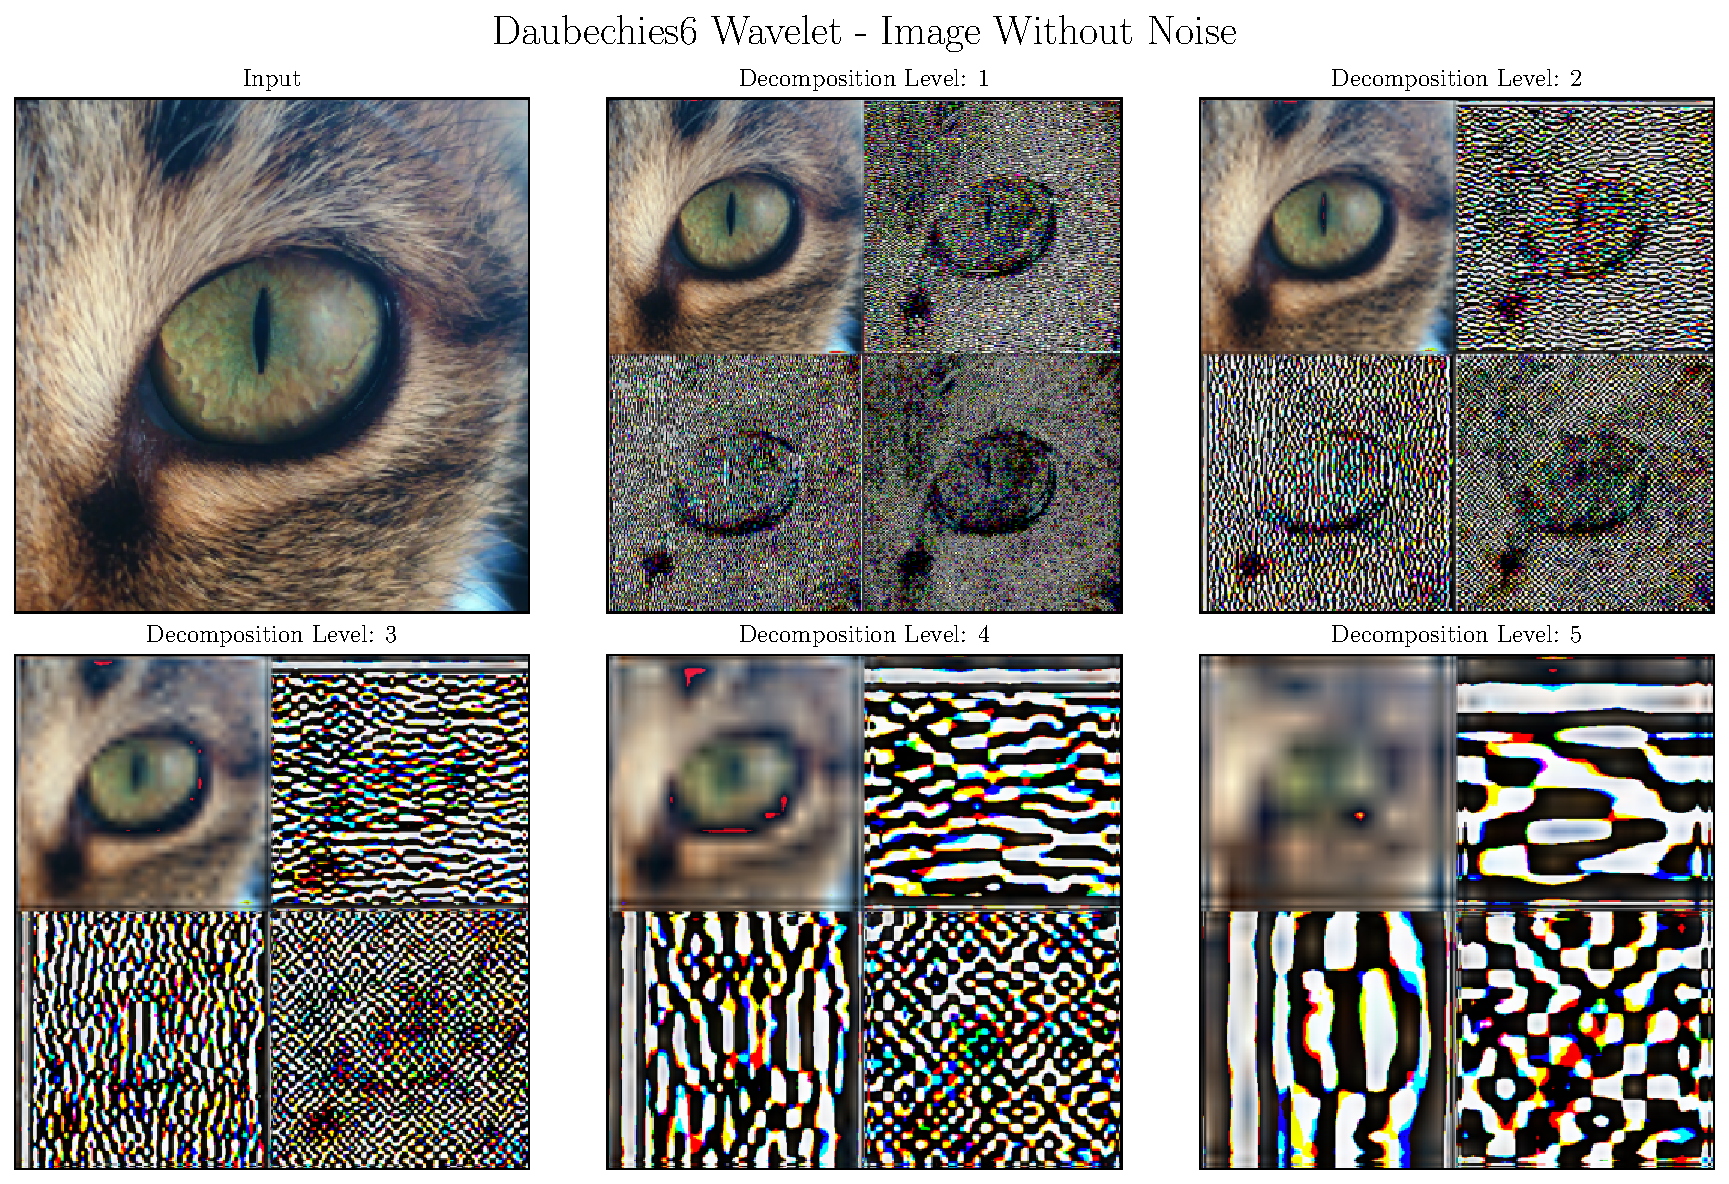
\includegraphics[height=7cm]{../Tests/Outputs/2D_Daubechies6Wavelet_WithoutNoise.pdf}
		\caption{Results of Daubechies6 wavelet on original image.}
		\label{fig:2d_db6}
	\end{figure}
	
	\begin{figure}[!h]
		\centering
		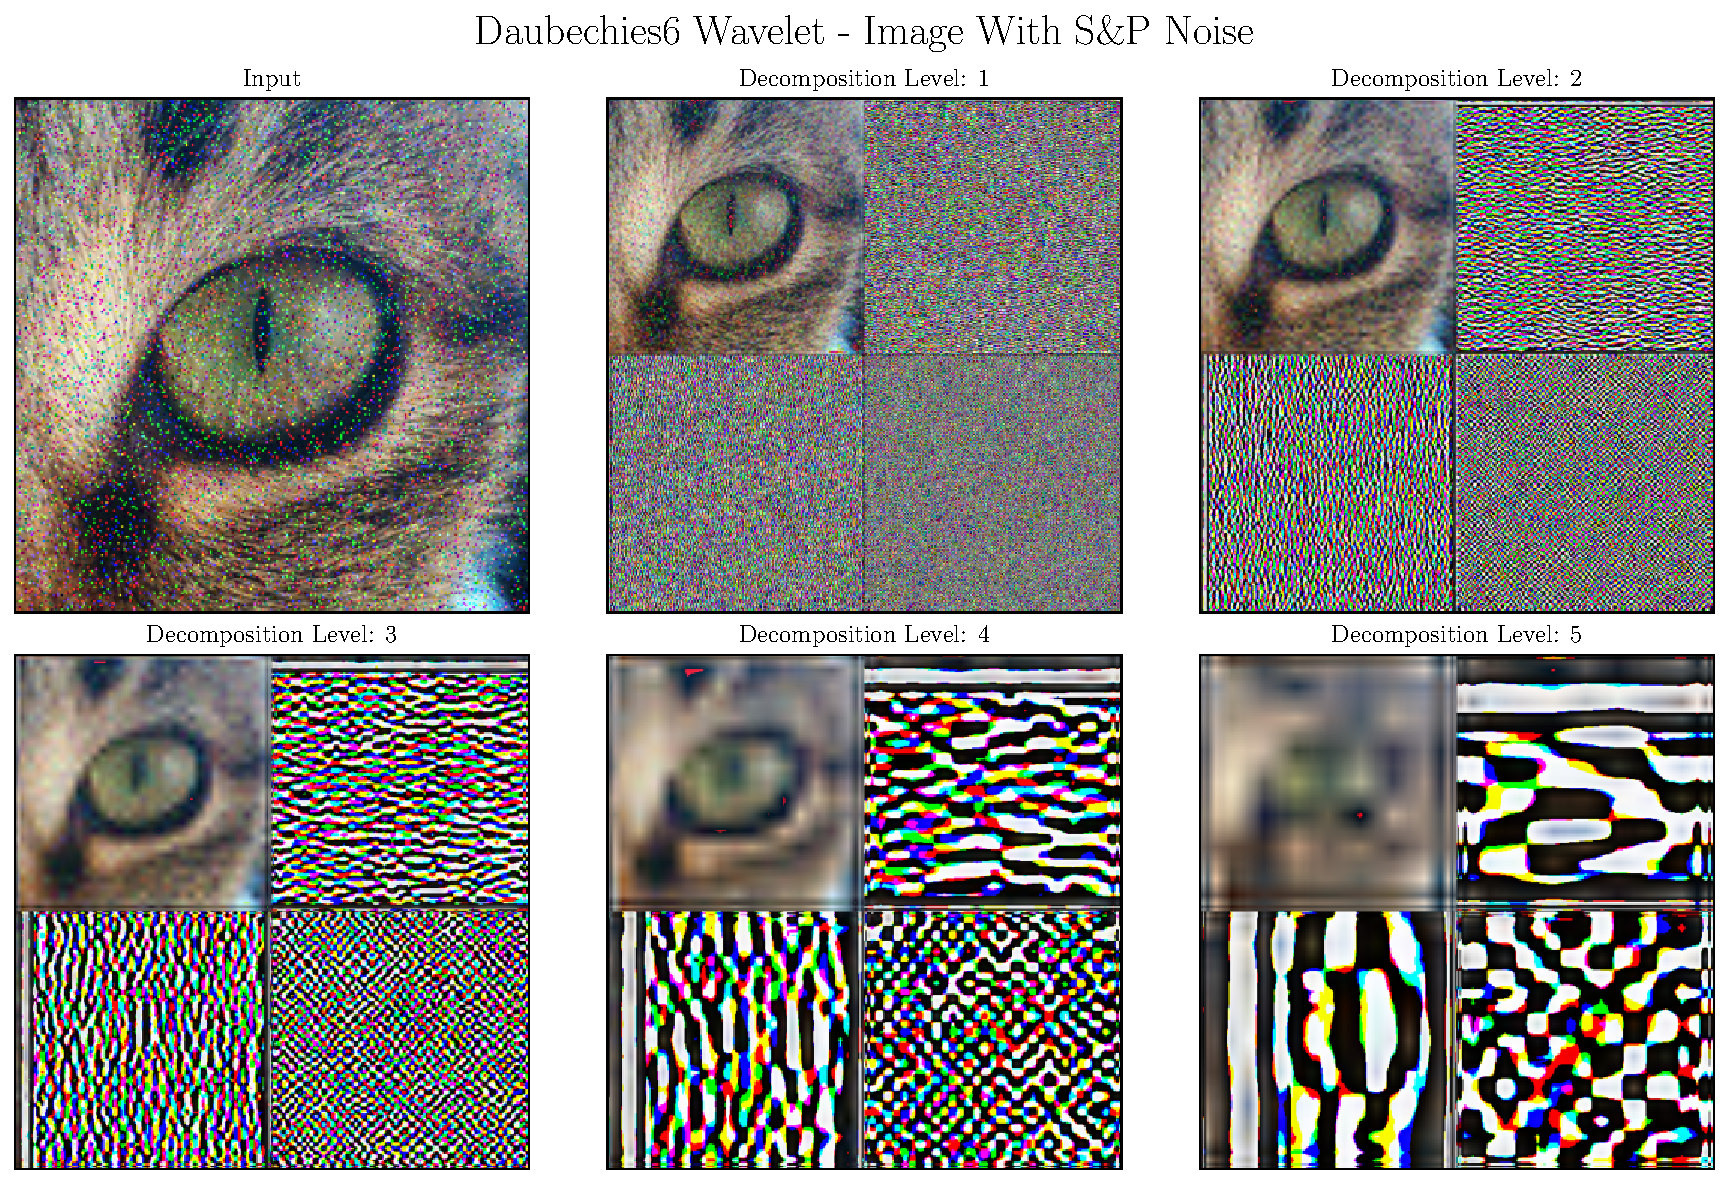
\includegraphics[height=7cm]{../Tests/Outputs/2D_Daubechies6Wavelet_SPNoise.pdf}
		\caption{Results of Daubechies6 wavelet on image with s\&p noise.}
		\label{fig:2d_db6_sp}
	\end{figure}
	
	\begin{figure}[!h]
		\centering
		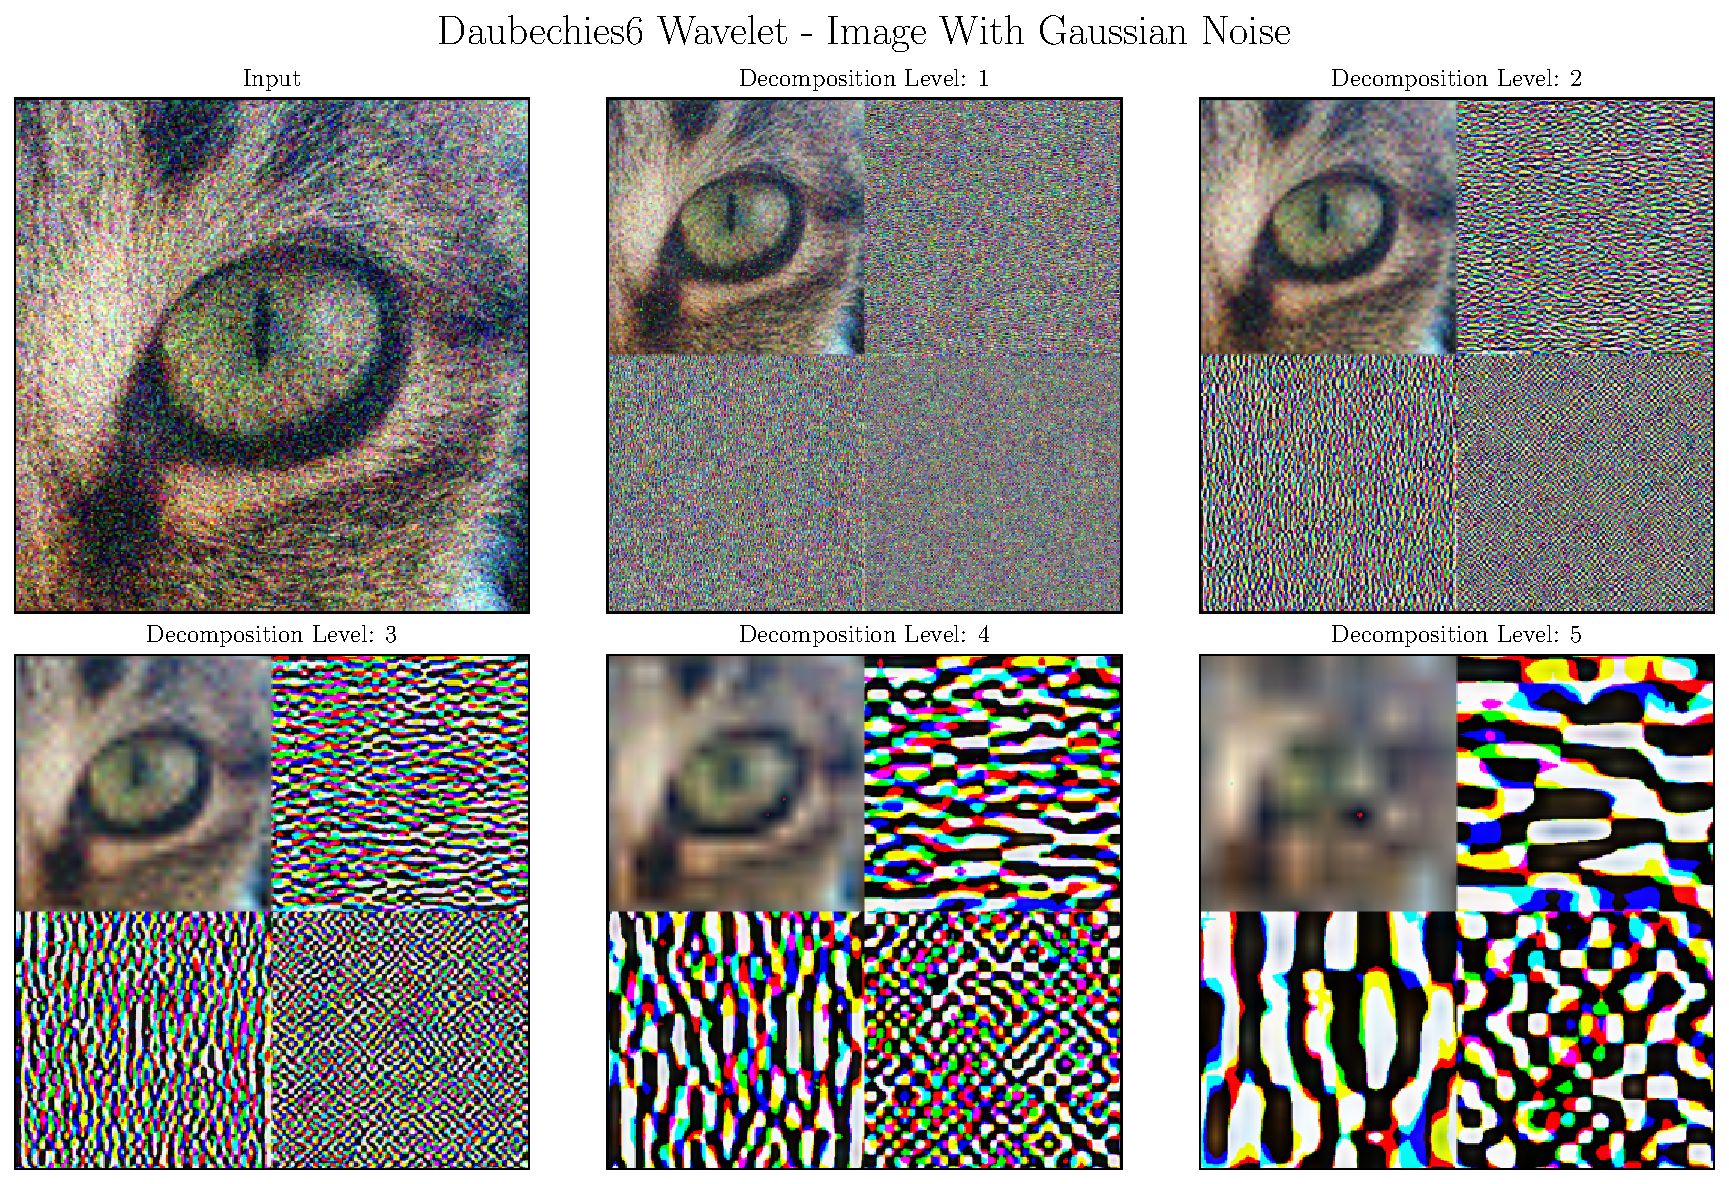
\includegraphics[height=7cm]{../Tests/Outputs/2D_Daubechies6Wavelet_GaussianNoise.pdf}
		\caption{Results of Daubechies6 wavelet on image with Gaussian noise.}
		\label{fig:2d_db6_gs}
	\end{figure}
	
	% Mexican Hat
	\begin{figure}[!h]
		\centering
		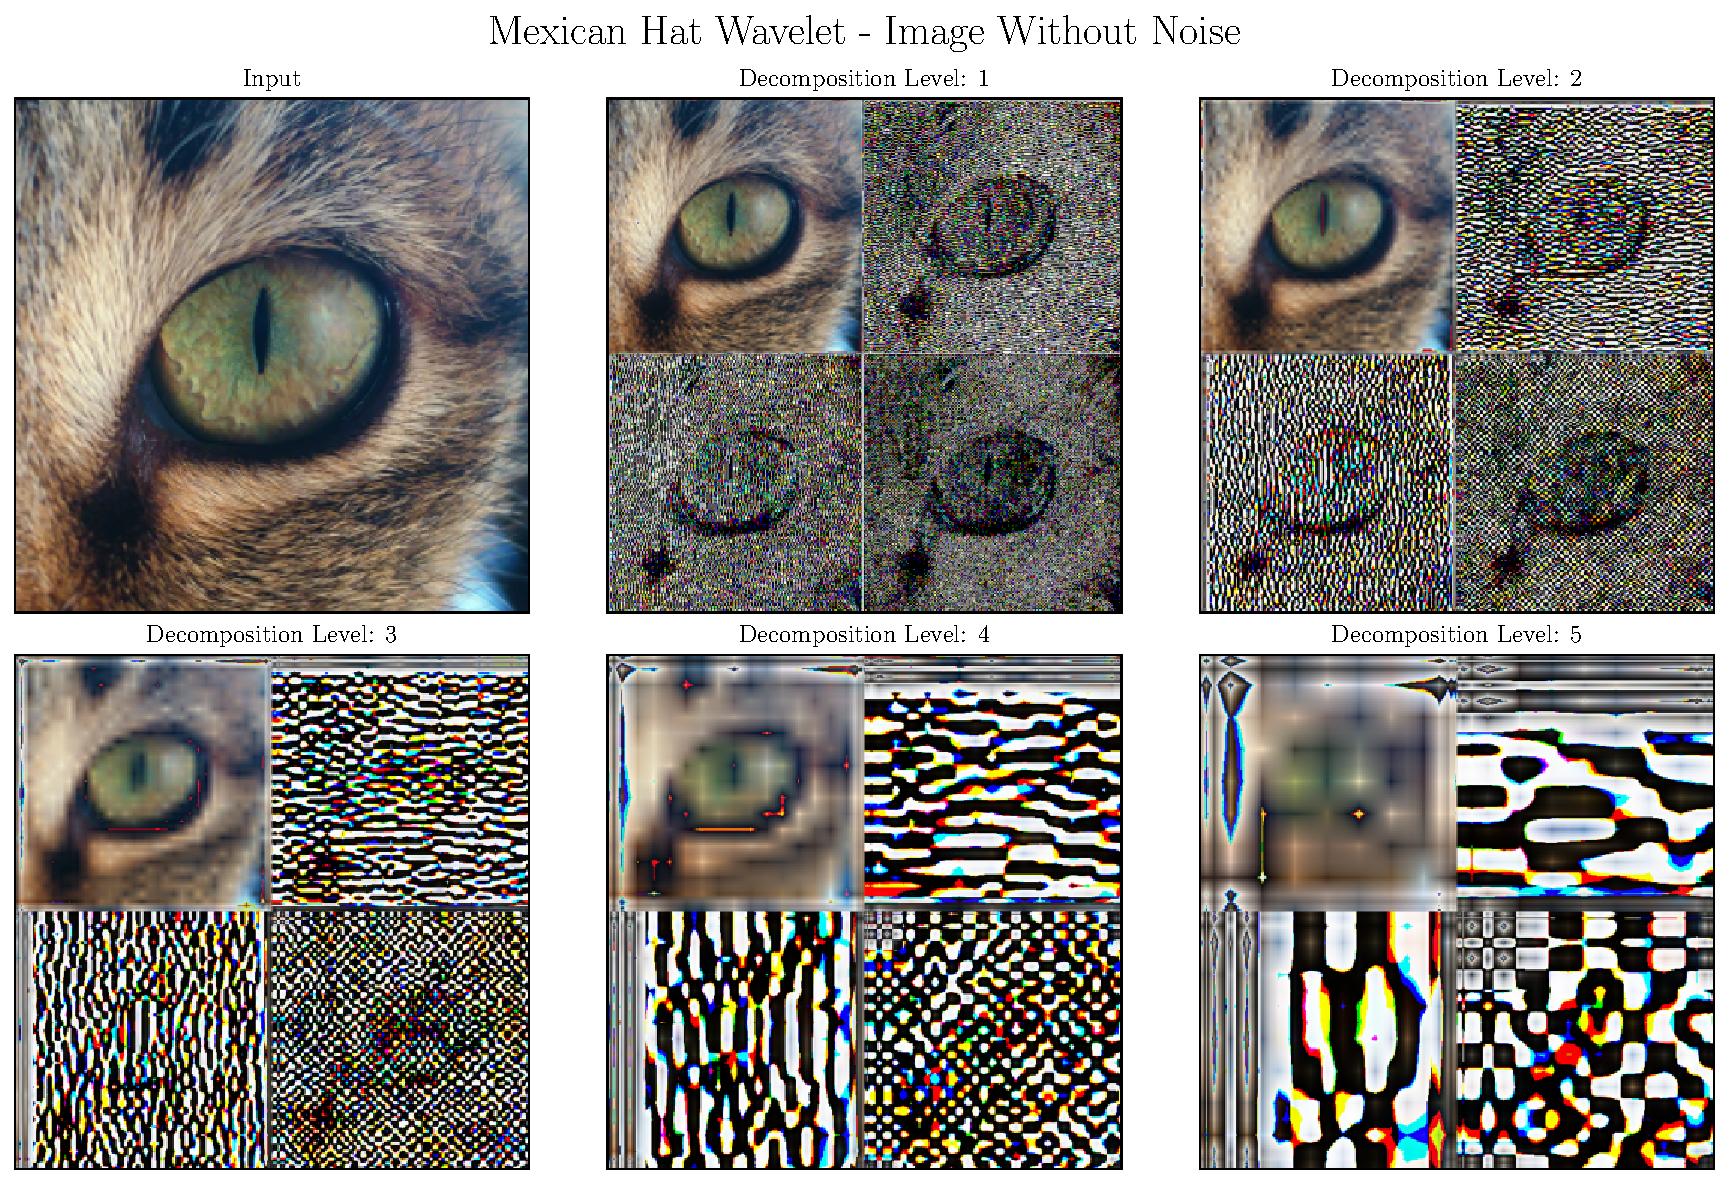
\includegraphics[height=7cm]{../Tests/Outputs/2D_MexicanHatWavelet_WithoutNoise.pdf}
		\caption{Results of Mexican Hat wavelet on original image.}
		\label{fig:2d_mh}
	\end{figure}
	
	\begin{figure}[!h]
		\centering
		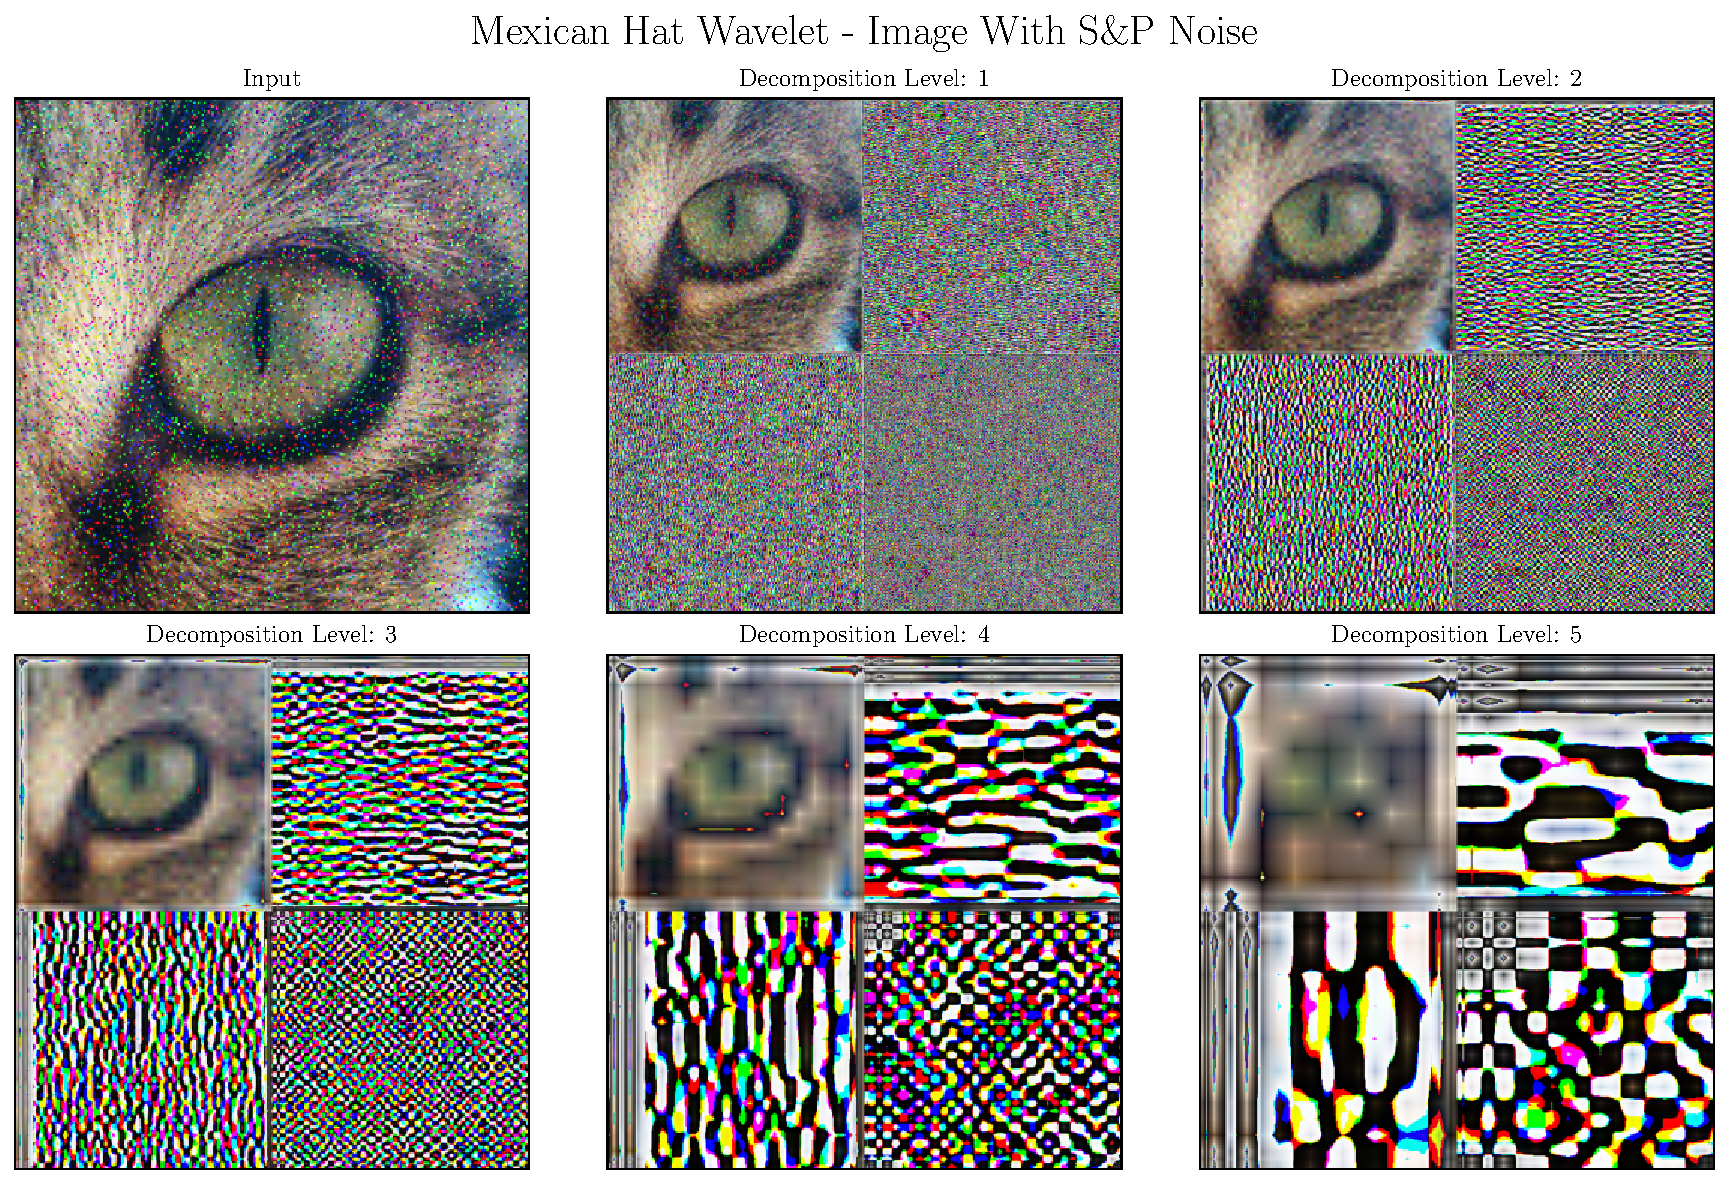
\includegraphics[height=7cm]{../Tests/Outputs/2D_MexicanHatWavelet_SPNoise.pdf}
		\caption{Results of Mexican Hat wavelet on image with s\&p noise.}
		\label{fig:2d_mh_sp}
	\end{figure}
	
	\begin{figure}[!h]
		\centering
		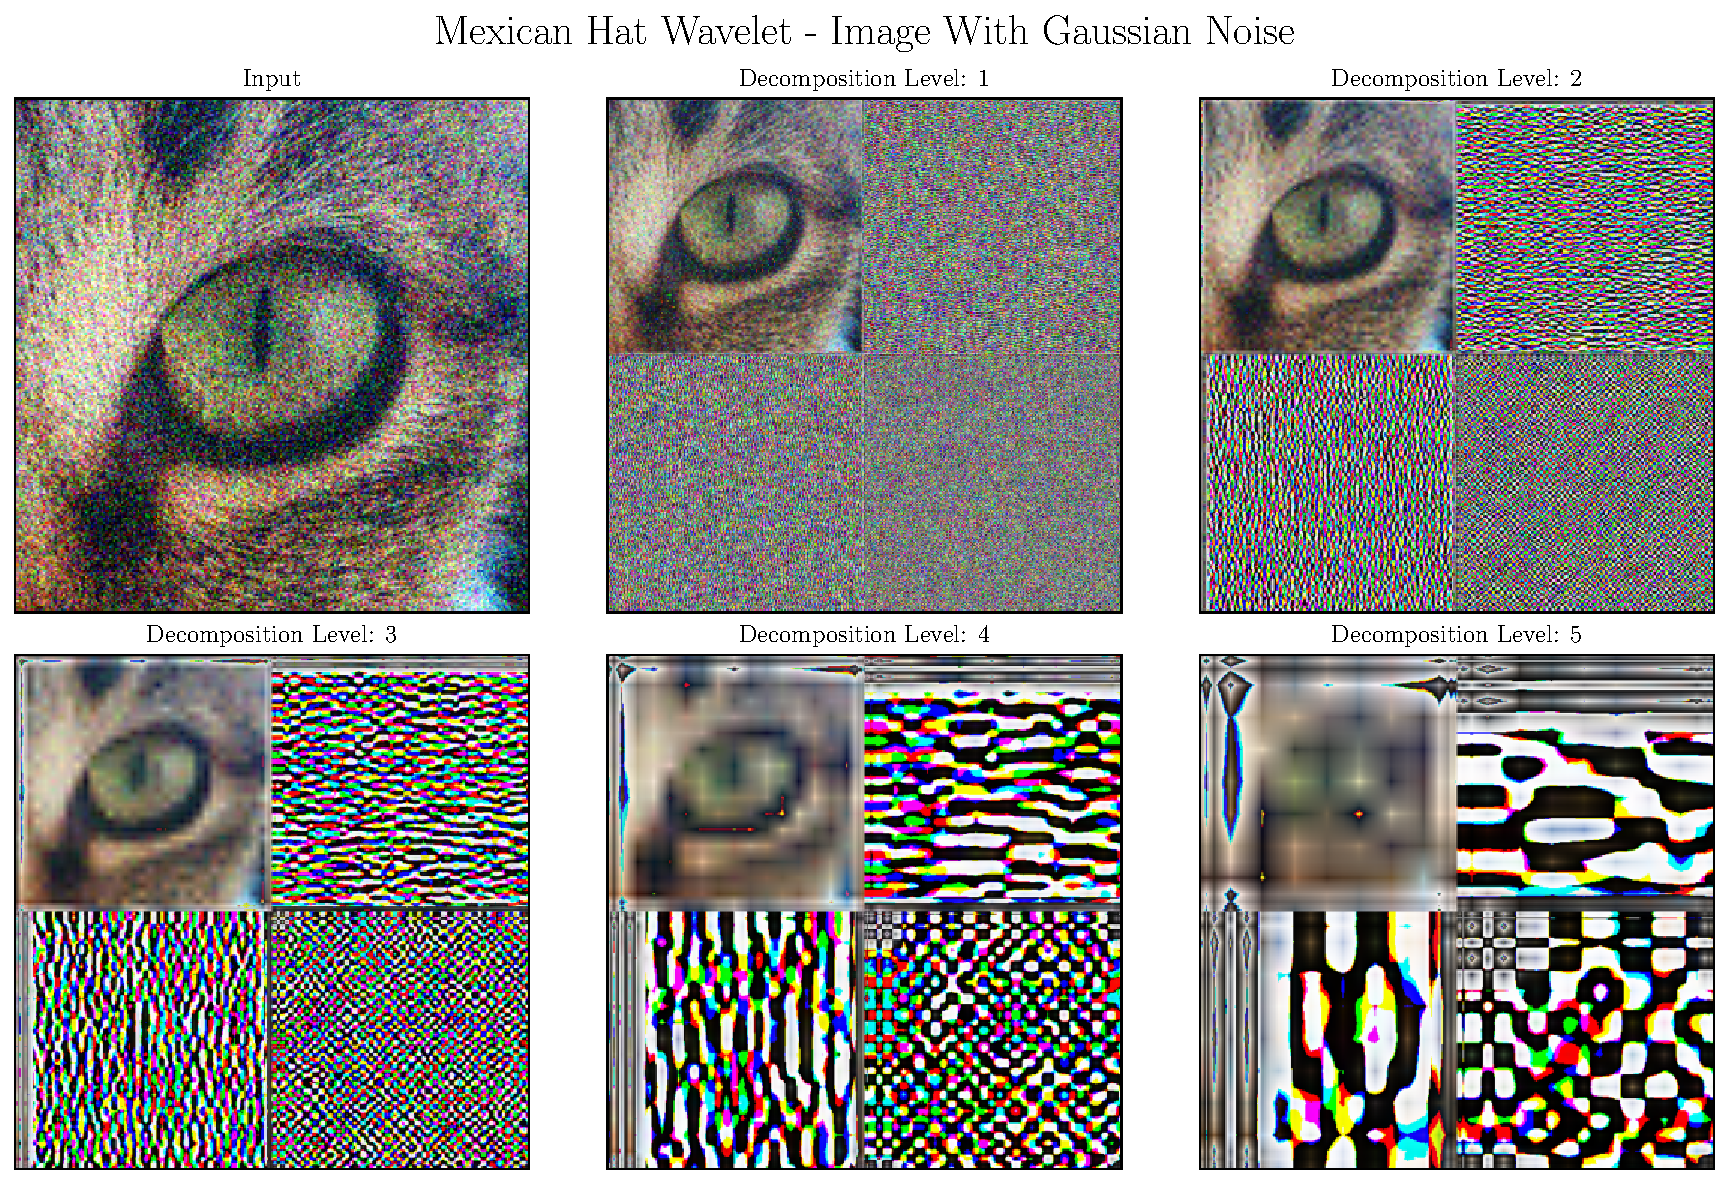
\includegraphics[height=7cm]{../Tests/Outputs/2D_MexicanHatWavelet_GaussianNoise.pdf}
		\caption{Results of Mexican Hat wavelet on image with Gaussian noise.}
		\label{fig:2d_mh_gs}
	\end{figure}
	
	% Symlet2
	\begin{figure}[!h]
		\centering
		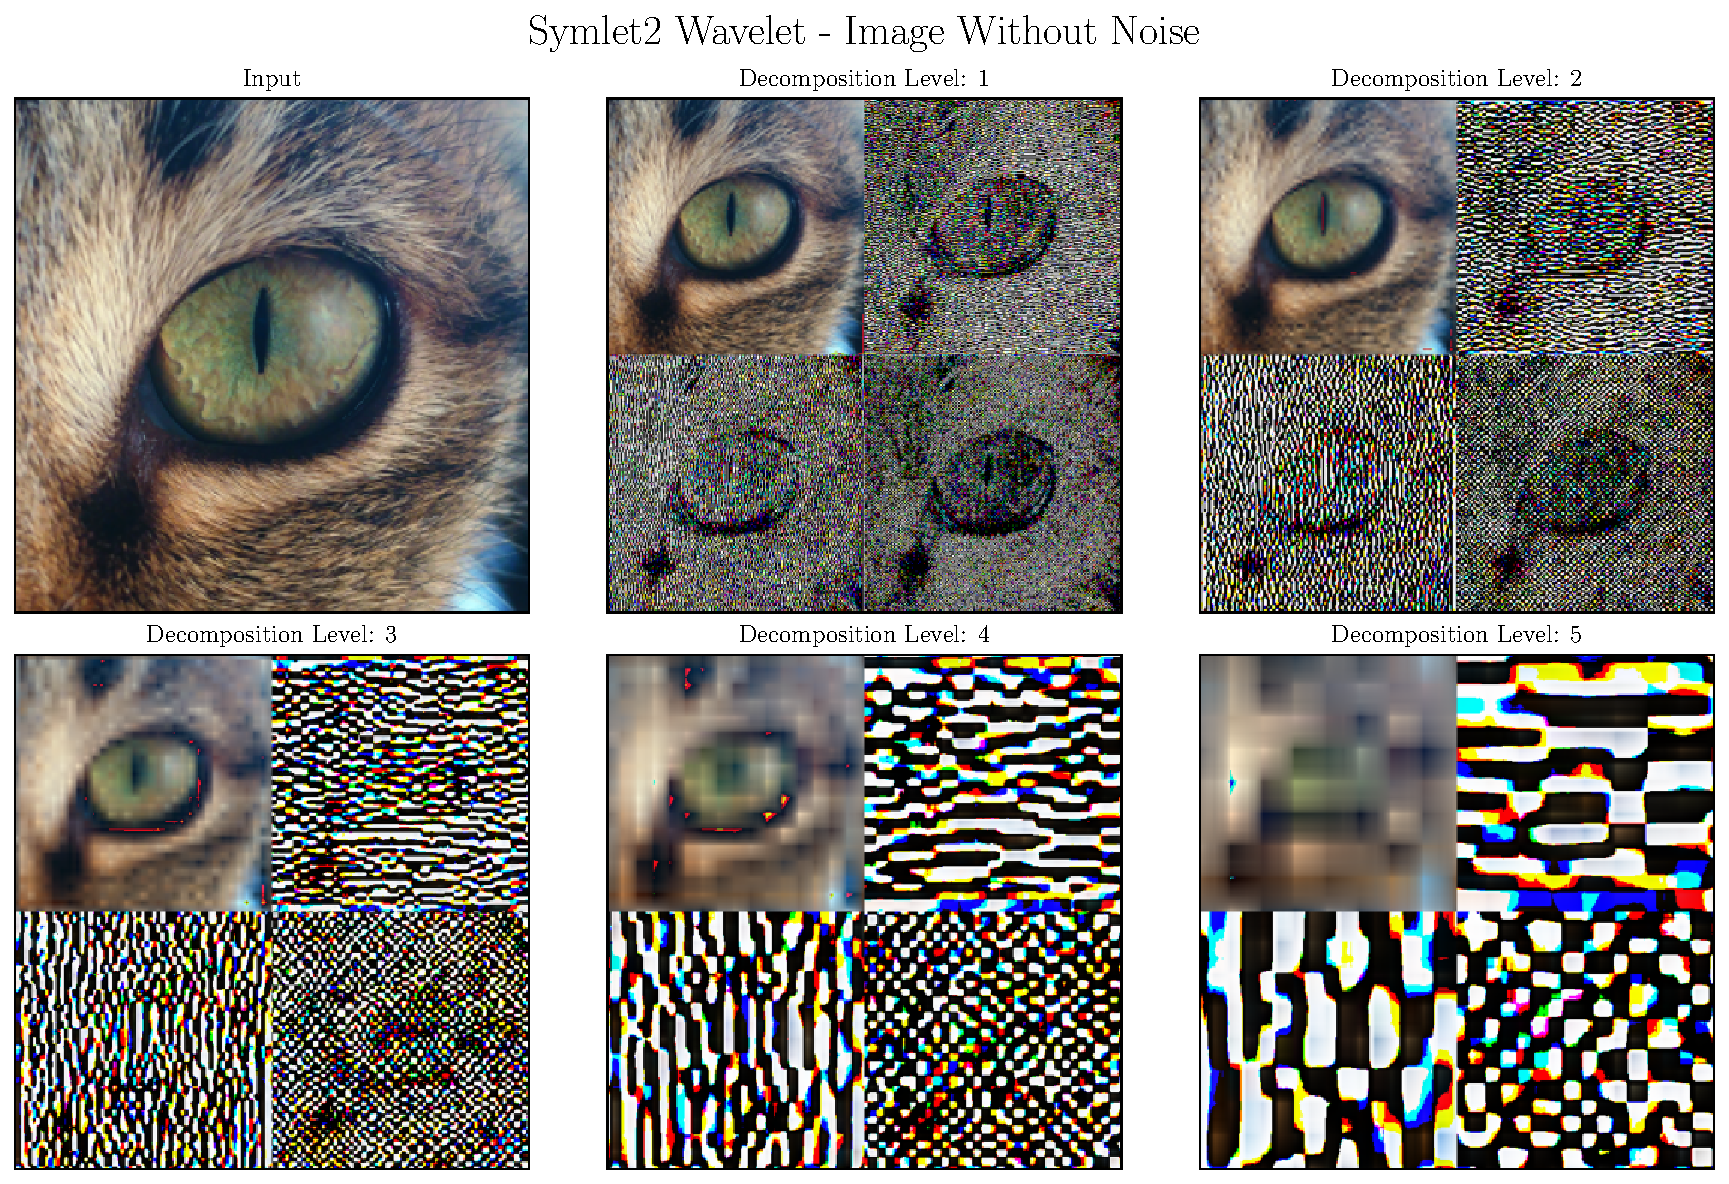
\includegraphics[height=7cm]{../Tests/Outputs/2D_Symlet2Wavelet_WithoutNoise.pdf}
		\caption{Results of Symlet2 wavelet on original image.}
		\label{fig:2d_sym2}
	\end{figure}
	
	\begin{figure}[!h]
		\centering
		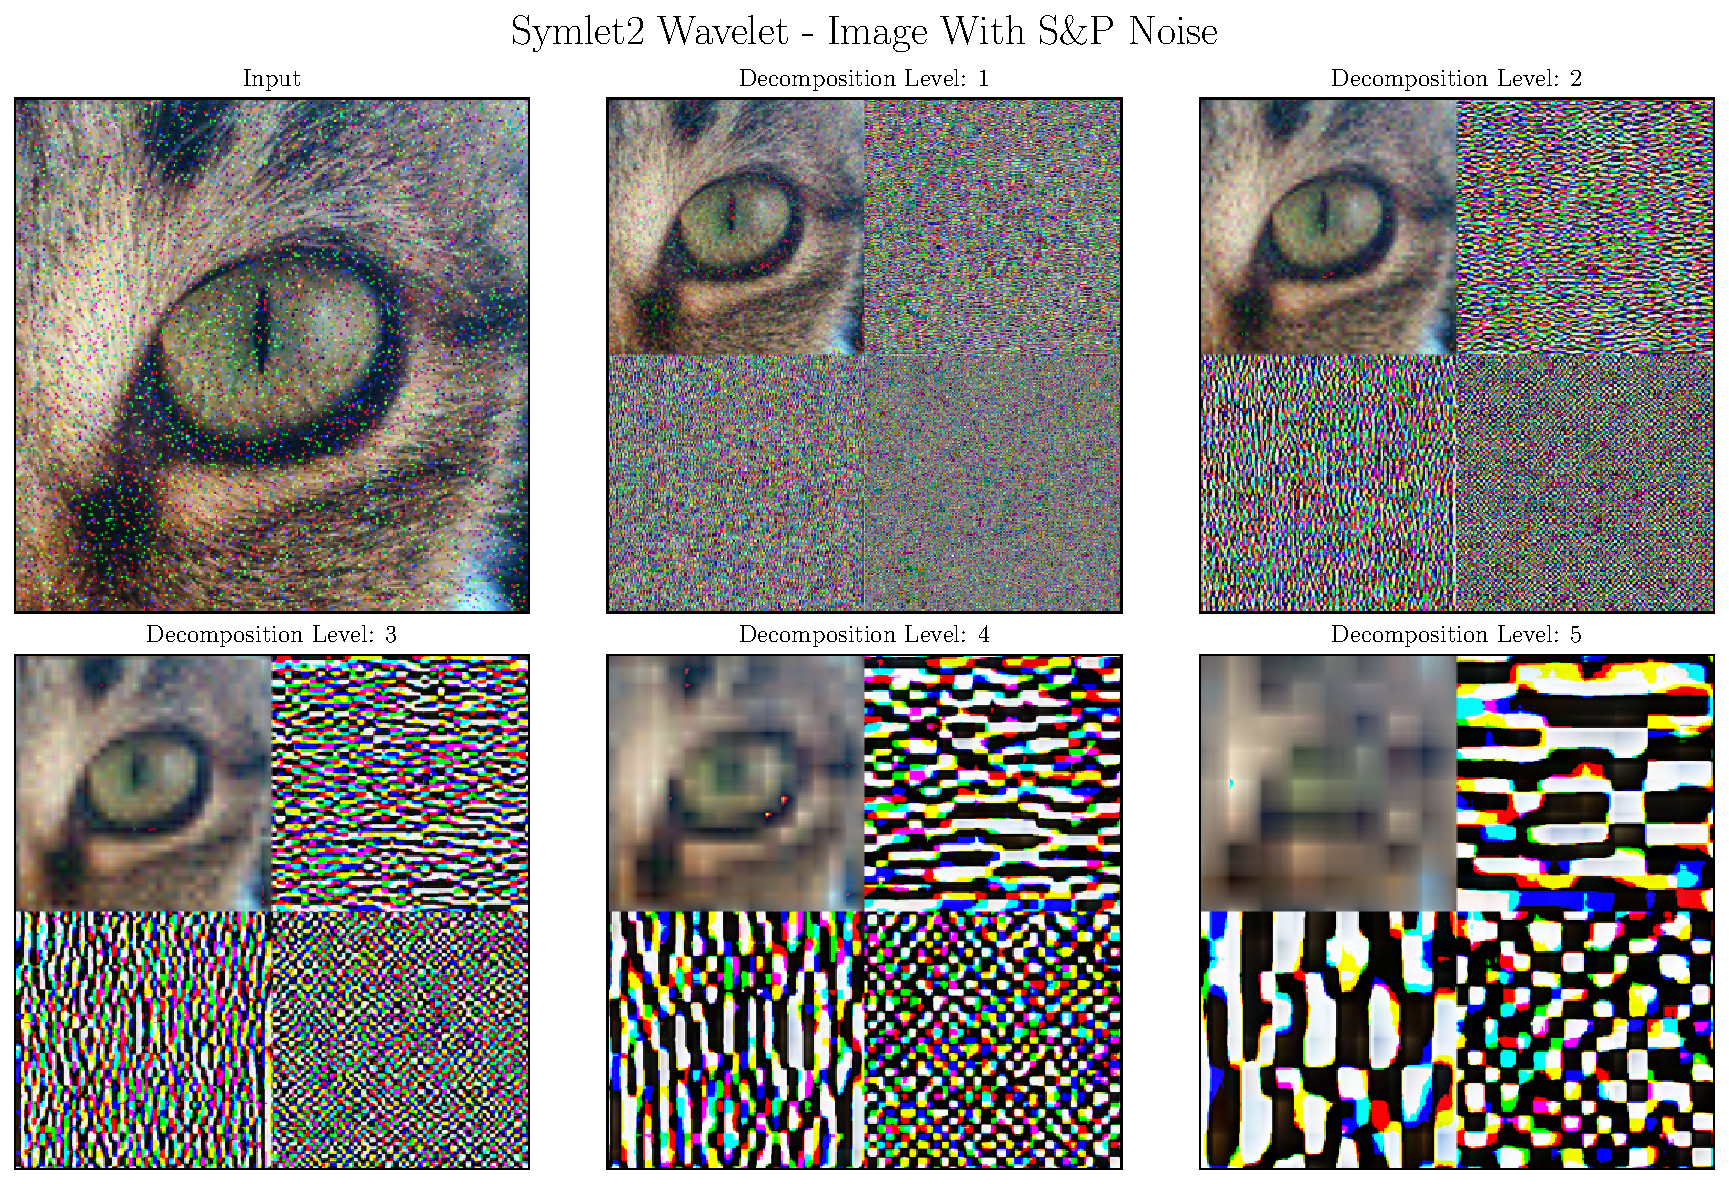
\includegraphics[height=7cm]{../Tests/Outputs/2D_Symlet2Wavelet_SPNoise.pdf}
		\caption{Results of Symlet2 wavelet on image with s\&p noise.}
		\label{fig:2d_sym2_sp}
	\end{figure}
	
	\begin{figure}[!h]
		\centering
		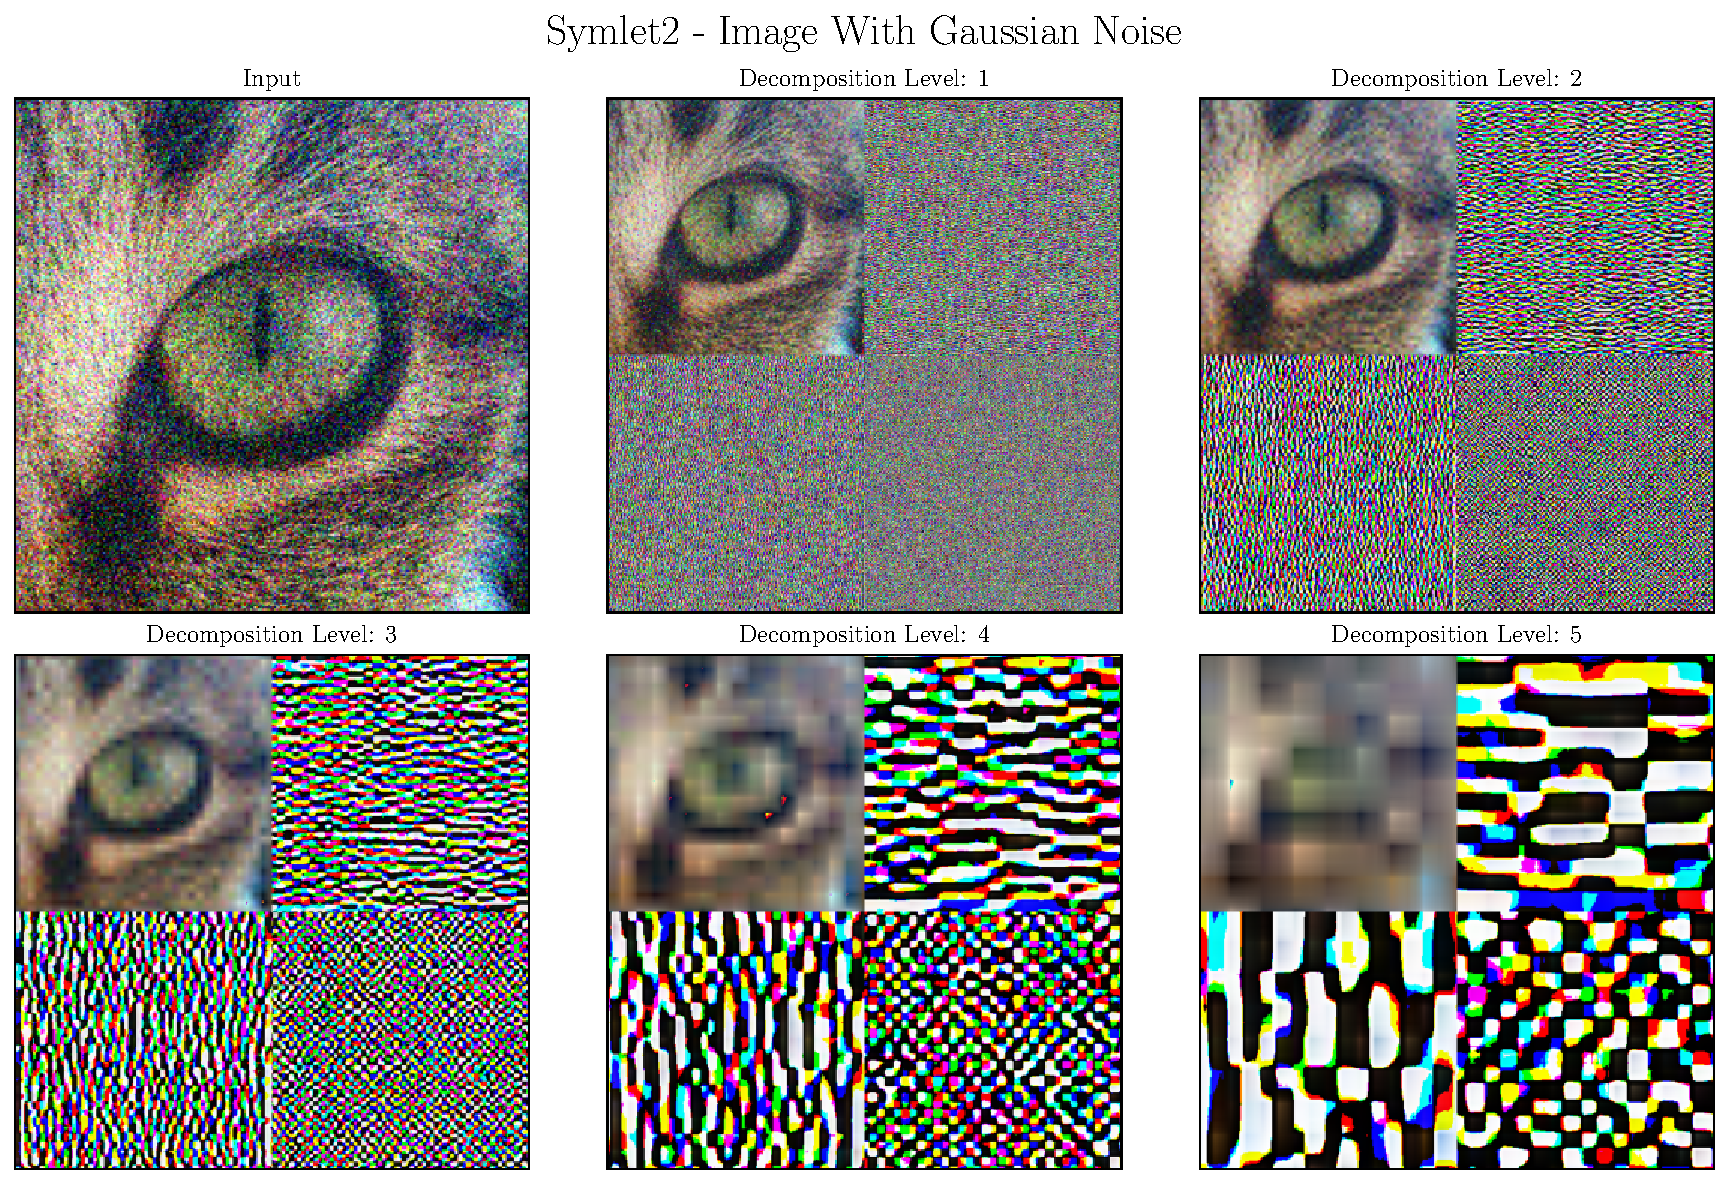
\includegraphics[height=7cm]{../Tests/Outputs/2D_Symlet2Wavelet_GaussianNoise.pdf}
		\caption{Results of Symlet2 wavelet on image with Gaussian noise.}
		\label{fig:2d_sym2_gs}
	\end{figure}
	\clearpage

\end{document}
